\documentclass[aspectratio=169,xcolor=table]{beamer}
\usetheme[style=classic]{mhar-vell}
%\usepackage{helvet}
%*--------------------------------------------------
\usepackage{bibunits}  
%\setbeamertemplate{bibliography item}{[\theenumiv]}
\setbeamertemplate{bibliography item}{\insertbiblabel}
\defaultbibliography{bibliography}
%\defaultbibliographystyle{IEEEtran}
%\defaultbibliographystyle{amsalpha}
\defaultbibliographystyle{abntex2-alf}
%\bibliography{bibliography}
%\usepackage[backend=biber,style=alphabetic,citestyle=authoryear]{biblatex}
% \addbibresource{bibliography.bib}
%\usepackage{natbib}
\usepackage{bibentry}
%*--------------------------------------------------
\usepackage{epigraph}
\usepackage{graphicx}
\usepackage{multirow}
%\usepackage{enumitem}
\usepackage{array}
%\usepackage{multimedia}
\usepackage{media9}
%\usepackage{pdfpc-movie}
\usepackage{tikz}
\usepackage{circledsteps}
\usepackage{listings}
\usepackage[normalem]{ulem}
%\usepackage{Sweave}
%\usepackage{xkeyval}
%\usepackage{palatino}
%\usepackage{pgfpages}
%*--------------------------------------------------
\usepackage[timeinterval=1]{tdclock}
%\usepackage[font=Times,timeinterval=1, timeduration=200,resetatpages=all]{tdclock}
%\usepackage[font=Times,timeinterval=10, timeduration=2.0, timedeath=0, fillcolorwarningsecond=white!60!yellow,timewarningfirst=50,timewarningsecond=80,resetatpages=2]{tdclock}
%*--------------------------------------------------
\usepackage{url}
\usepackage{tabularx,booktabs}
\usepackage{threeparttable}
\usepackage[absolute, overlay]{textpos}
%*--------------------------------------------------
\usepackage{framed, color}
\usepackage[tikz]{bclogo}
\usepackage{spot}
\setspotlightcolor{red!50}
% %\setspotlightstyle{star, fill=red!50}
% %\setspotlightstyle{star points=7}
\usepackage{color,soul}
%\usepackage{xcolor}
\usepackage{tcolorbox}
\usepackage{xcolor}
%*--------------------------------------------------
\usepackage{amsmath}
\usepackage{xfrac}
\usepackage{units}
\usepackage{ulem}
%*-------------------------------------------------------------------------------
%\newcolumntype{C}[1]{>{\centering\arraybackslash}m{#1}}
\newcolumntype{L}[1]{>{\raggedright\let\newline\\\arraybackslash\hspace{0pt}}m{#1}}
\newcolumntype{C}[1]{>{\centering\let\newline\\\arraybackslash\hspace{0pt}}m{#1}}
\newcolumntype{R}[1]{>{\raggedleft\let\newline\\\arraybackslash\hspace{0pt}}m{#1}}
%*-------------------------------------------------------------------------------
%\pgfpagesuselayout{2 on 1}[a4paper,border shrink=5mm]
%\setbeamertemplate{note page}[plain]
%\setbeameroption{show notes on second screen=bottom}
%*-------------------------------------------------------------------------------
\setbeameroption{hide notes}
%\setbeameroption{show only notes}
%\setbeameroption{show notes on second screen=right}
\setbeamertemplate{note page}{\pagecolor{yellow!5}\insertnote}
%*-------------------------------------------------------------------------------
\title              {Método BiLi}
\subtitle           {Otimização para revisão bibliográfica}
\author             {Marco Reis}
\email              {marcoreis@fieb.org.br}
\advisor            {Orientador: Roberto L. S. Monteiro}
\institute          {Robótica e Sistemas Autônomos, Senai Cimatec}
\date               {Outubro de 2021}
% \ulogo        		{Template/logosenaicimatecnegativo}
% \ulogof             {Template/logosenaicimatec2020}
% \ulogoo        		{Template/rosa-logo}
% \ulistelement    	{Template/bullet-white}

%*-------------------------------------------------------------------------------
\graphicspath{{Source/pictures/}}
%*-------------------------------------------------------------------------------
\totalNoSlidesDisabled % To turn off the total number of slides in the footer. Comment this if you want the total number of slides in the footer
%*-------------------------------------------------------------------------------
\begin{document}
%*----------- COVER -------------------------------------------------------------
\begin{frame}[t,plain]
%*----------- sound--------------------------------
    \includemedia[
        width=1ex,
        height=1ex,
        %activate=pageopen, 
        activate=onclick,
        deactivate=onclick,
        %passcontext,
        transparent,
        addresource=./Source/sounds/hip-hop.mp3,
        flashvars={
                    source=./Source/sounds/hip-hop.mp3
                    %&autoPlay=true
                    &autoRewind=true
                    &Play=2s
                    &repeat=always
                    %&Loop=true
        }
    ]
    {}{VPlayer.swf}
%*----------- start-page--------------------------
    \titlepage
%*----------- notes-------------------------------
    \note[item]{Notes can help you to remember important information. Turn on the notes option.}
    \note[item]{Notes can help you to remember important information. Turn on the notes option.}
\end{frame}
%-
%*----------- SECTIONS ----------------------------------------------------------
%*----------- SLIDE -------------------------------------------------------------
\begin{frame}[t]{A pesquisa na vida real} 
    \transdissolve[duration=0.5]
    A complexidade do conhecimento nas inovações tem aumentado ano após ano. A necessidade do ser humano em alcançar patamares cada vez mais eficientes em nosso dia a dia, faz com que tenhamos cada vez mais uma capacidade de otimização na busca por conhecimento.

    \centering
    \vspace*{0.1cm}
    \Large{O tempo é vital.}

    \roundpic[xshift=0cm,yshift=0cm]{4cm}{7cm}{time}
    %\newline

        % \begin{columns}[t]
        %     \column{.05\linewidth}
        %     \column{.4\linewidth}
        %         \huge{O tempo é vital.}
        %     \column{.6\linewidth}
        %     \begin{center}
        %     %\centerline{
        %         \begin{figure}
        %             %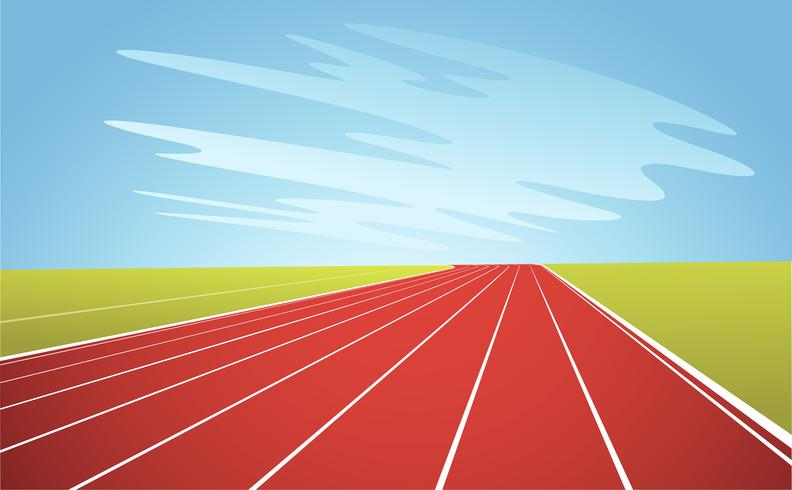
\includegraphics[width=1\textwidth]{pista}
        %             %\caption{Pista de corrida \cite{agostini2007}}
        %             \roundpic[xshift=0cm,yshift=0cm]{4cm}{7cm}{time}
        %             %\caption{Pista de corrida \cite{agostini2007}}
        %         \end{figure}
        %     %}
        %     \end{center}
        % \end{columns}
%*----------- notes
    \note[item]{Notes can help you to remember important information. Turn on the notes option.}
\end{frame}
%-
%*----------- SLIDE -------------------------------------------------------------
\begin{frame}[c]{Como vocês realizam as buscas por artigos?} 
    \transdissolve[duration=0.5]
   
    \begin{center}
        \Wider{%
        \begin{shaded}
        \begin{center}
            \vspace*{0.5cm}
            \resizebox{!}{0.7cm}{%
                \textcolor{cyan}{G}\textcolor{red}{o}\textcolor{orange}{o}\textcolor{cyan}{g}\textcolor{teal}{l}\textcolor{red}{e}?
            }%
        \end{center}
        \end{shaded}
        }%
    \end{center}
%*----------- notes
    \note[item]{Notes can help you to remember important information. Turn on the notes option.}
\end{frame}
%-
%*----------- SLIDE -------------------------------------------------------------
\begin{frame}[c]{Como vocês realizam as buscas por artigos?} 
    \transdissolve[duration=0.5]
   
    \centering
    
\includegraphics[clip, trim = 0 0 0 0,  width=.83\textwidth]{databases.jpg}
%*----------- notes
    \note[item]{Notes can help you to remember important information. Turn on the notes option.}
\end{frame}
%-
%*----------- SLIDE -------------------------------------------------------------
\begin{frame}[c]{Como vocês realizam as buscas por artigos?} 
    \framesubtitle{Pouco tempo para muito resultado}
    \transdissolve[duration=0.5]
   
    \centering
    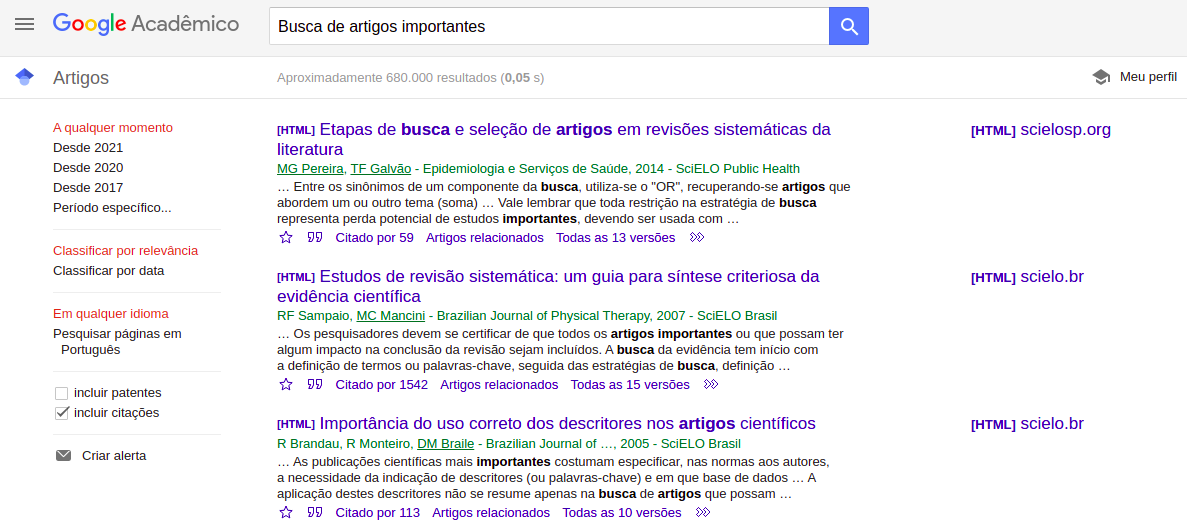
\includegraphics[clip, trim = 0 0 0 0,  width=1\textwidth]{googleacademico2.png}
%*----------- notes
    \note[item]{Notes can help you to remember important information. Turn on the notes option.}
\end{frame}
%-
%*----------- SLIDE -------------------------------------------------------------
\begin{frame}[c]{Como vocês realizam as buscas por artigos?} 
    \framesubtitle{Pouco tempo para muito resultado}
    \transdissolve[duration=0.5]
   
    \centering
    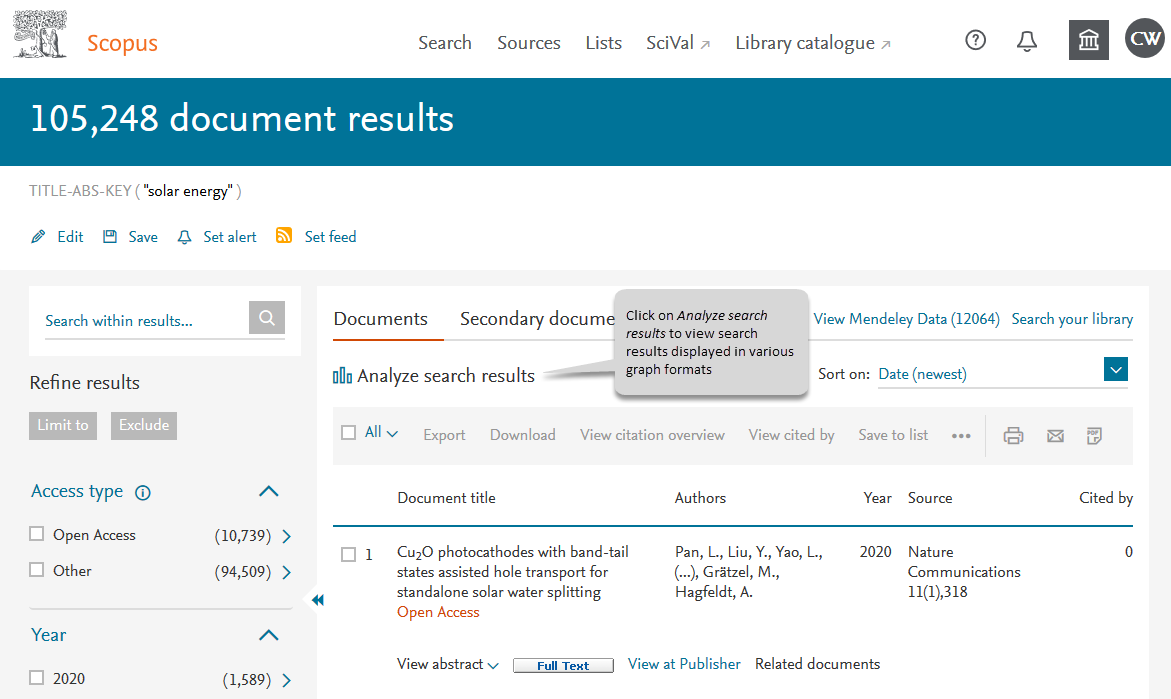
\includegraphics[clip, trim = 0 0 0 0,  width=.75\textwidth]{scopus.png}
%*----------- notes
    \note[item]{Notes can help you to remember important information. Turn on the notes option.}
\end{frame}
%-
%*----------- SLIDE -------------------------------------------------------------
\begin{frame}[c]{Como vocês realizam as buscas por artigos?} 
    \framesubtitle{Pouco tempo para muito resultado}
    \transdissolve[duration=0.5]
   
    \centering
    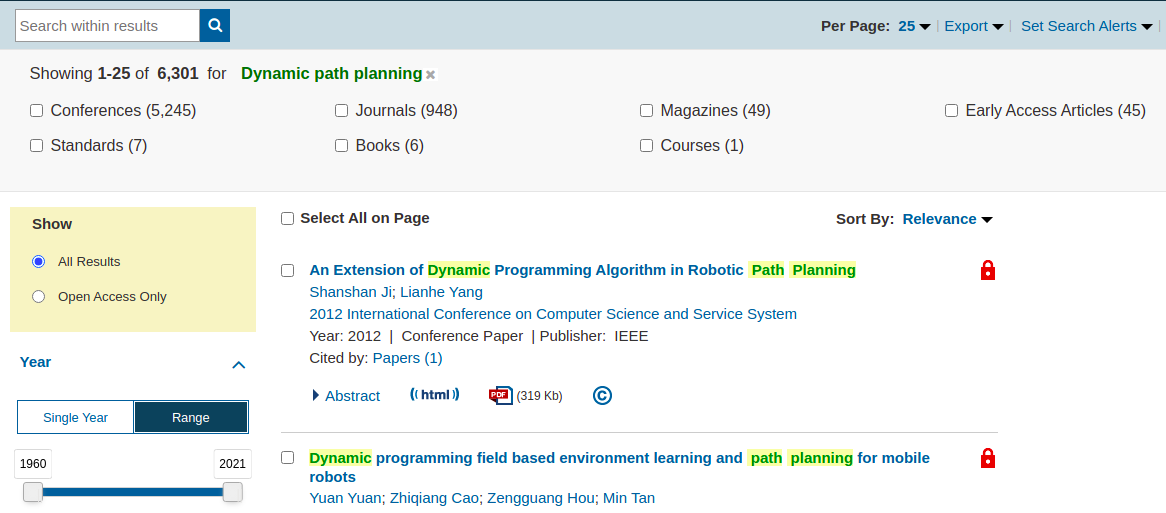
\includegraphics[clip, trim = 0 0 0 0,  width=1\textwidth]{ieee.png}
%*----------- notes
    \note[item]{Notes can help you to remember important information. Turn on the notes option.}
\end{frame}
%-
%*----------- SLIDE -------------------------------------------------------------
\begin{frame}[t]{Tempo e precisão}
    \transboxout[duration=0.5]
    %\framesubtitle{Darwin-OP}
    Uma das vertentes da tecnologia é a capacidade de tornar os processos mais rápidos e precisos, suportando a vida humana no planeta.

    \vspace*{0.2cm}
    Alguns fatores impulsionadores
		\begin{itemize}
			\item Competitividade
			\item Prazo de entrega
			\item Concluir um trabalho 
		\end{itemize}

    \vspace*{0.2cm}
    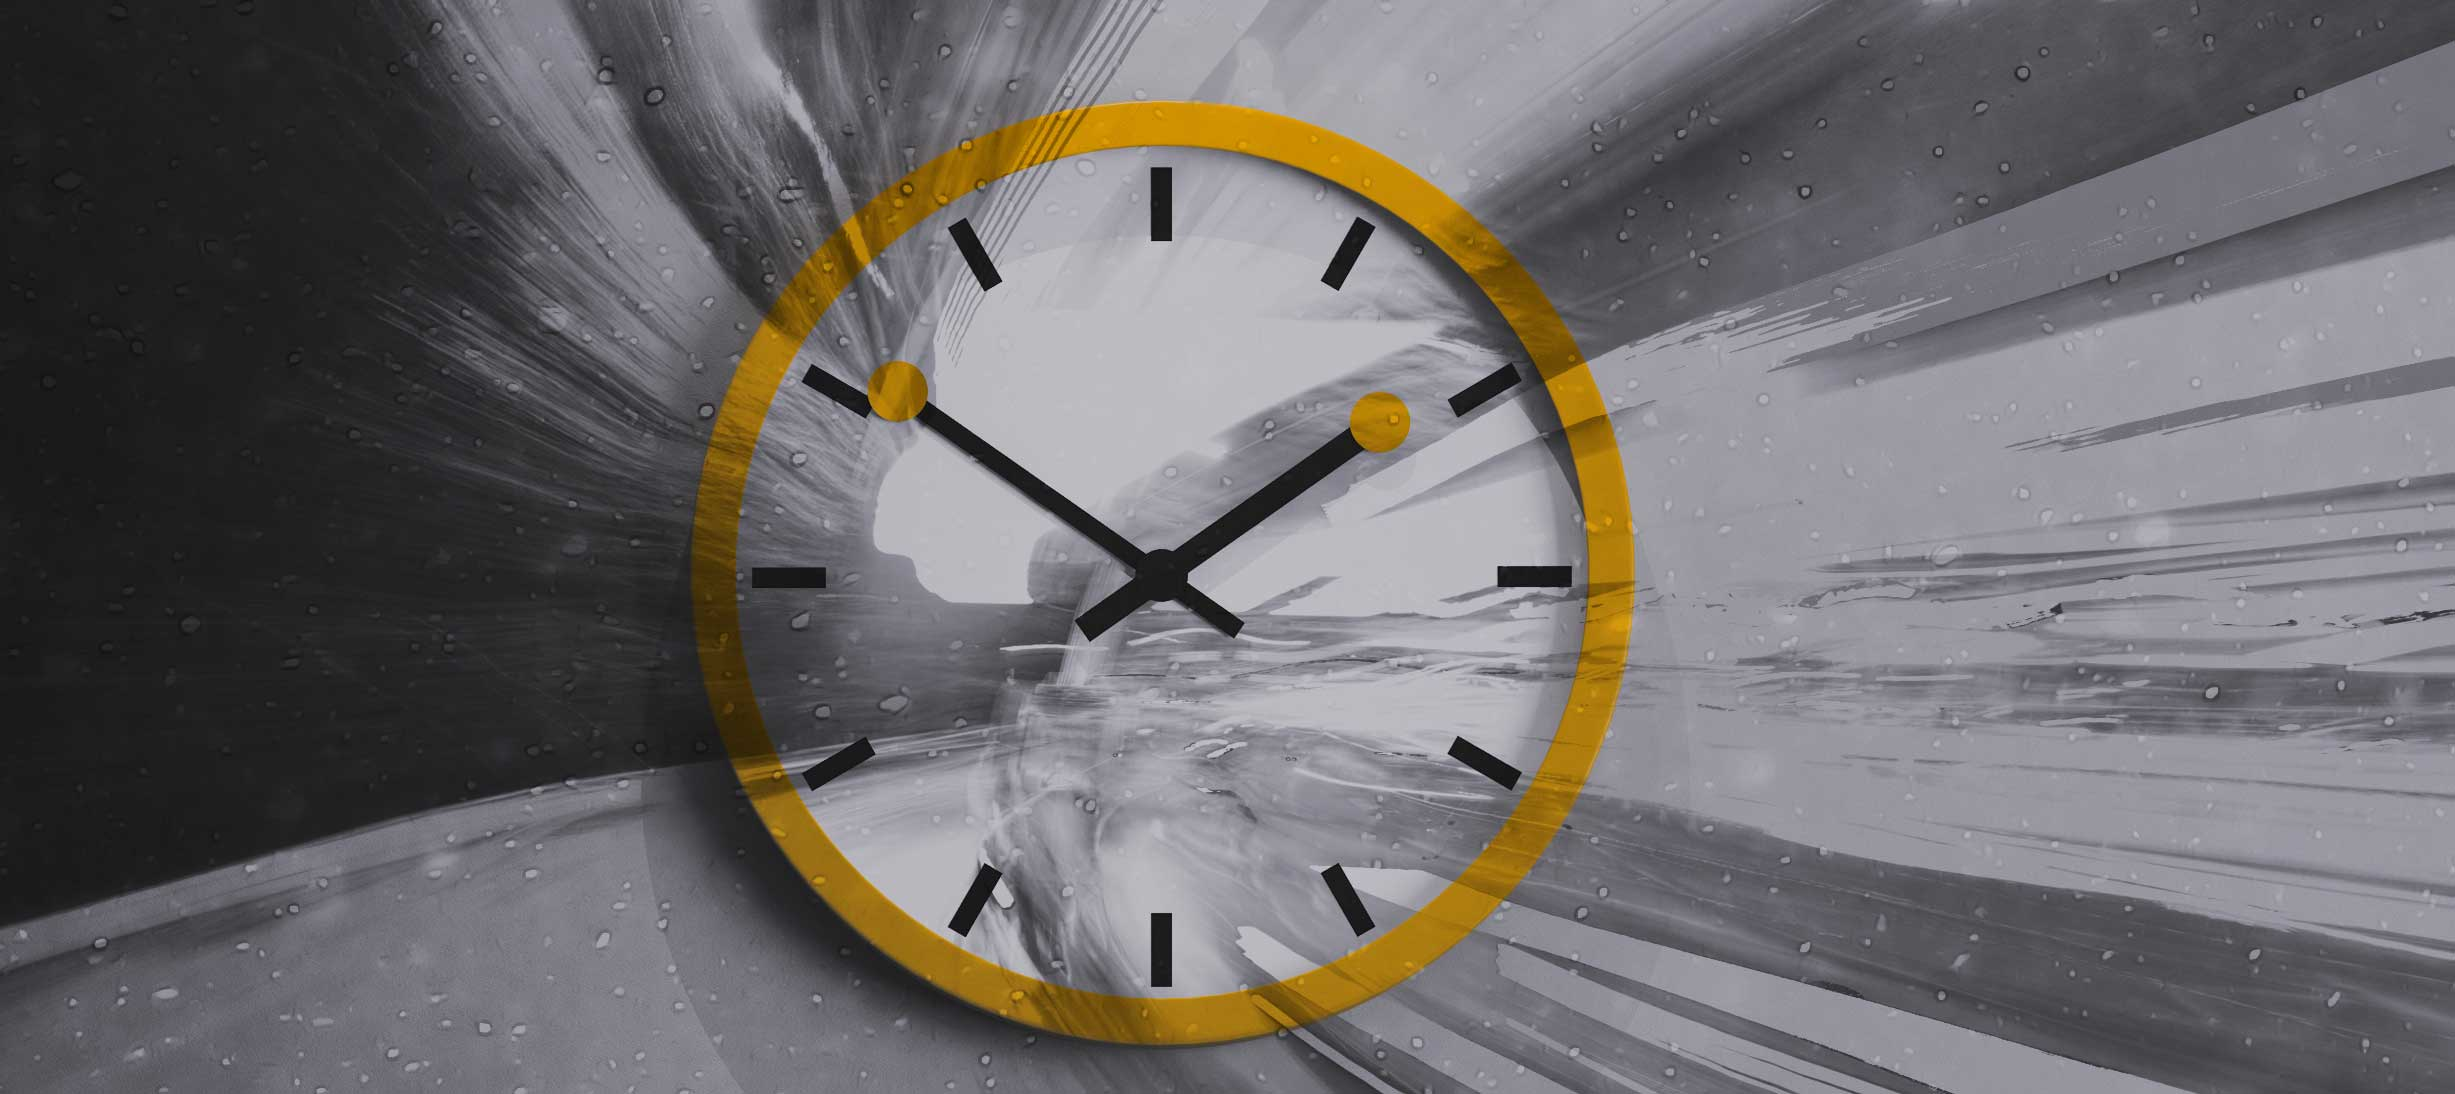
\includegraphics[clip, trim = 0 420 0 80, width=1\textwidth]{time-and-precision.jpeg}

    \begin{columns}
        \column{.1\textwidth}
        \column{.5\textwidth}
        \column{.4\textwidth}
    \end{columns}
%*----------- notes
    \note[item]{Notes can help you to remember important information. Turn on the notes option.}
\end{frame}
%-
%*----------- SLIDE -------------------------------------------------------------
\begin{frame}[t]{As ferramentos para aceleração} 
    \transdissolve[duration=0.5]

    % \roundpic[xshift=0cm,yshift=0cm]{4cm}{7cm}{time}


        \begin{columns}[t]
            \column{.05\linewidth}
            \column{.4\linewidth}
                \begin{enumerate}
                    \item conta no \href{https://colab.research.google.com/}{Google Colab}
                    \item \href{https://www.rstudio.com/products/rstudio/}{RStudio} (R $\geq$ 3.5)
                    \item R-package \href{https://www.bibliometrix.org/}{Bibliometrix}
                    \item R-package \href{https://elizagrames.github.io/litsearchr/}{LitSearchr}
                    \item R-package \href{https://revtools.net/}{RevTools}
                    \item \href{https://www.mendeley.com/?interaction_required=true}{Mendeley}
                    \item \href{https://cmap.ihmc.us/}{CMapTools}
                \end{enumerate}
            \column{.6\linewidth}
                % \begin{center}
                \centering
                \begin{figure}
                         
\includegraphics[width=0.5\textwidth]{colab.png}
                %         %\caption{Pista de corrida \cite{agostini2007}}
                %         %\roundpic[xshift=0cm,yshift=0cm]{4cm}{7cm}{time}
                %         %\caption{Pista de corrida \cite{agostini2007}}
                \end{figure}
                \href{https://colab.research.google.com/drive/1DP0-hgr_tXYGTs2M-9NrsMy8NsUi1hwt?usp=sharing}{bili-method.ipynb}

                
        
                % \end{center}
        \end{columns}
%\href{https://colab.research.google.com/drive/1DP0-hgr_tXYGTs2M-9NrsMy8NsUi1hwt#scrollTo=EDGnoWZD8Cvl&line=5&uniqifier=1}{link-to-colab}
%*----------- notes
    \note[item]{Notes can help you to remember important information. Turn on the notes option.}
\end{frame}
%-

%*----------- SLIDE -------------------------------------------------------------
\begin{frame}[t]{Melhoria na busca de artigos}
    \framesubtitle{Existe algum método eficiente?}
    %\transboxin[duration=1,direction=30]
    A biblioteconomia.

    \begin{figure}
        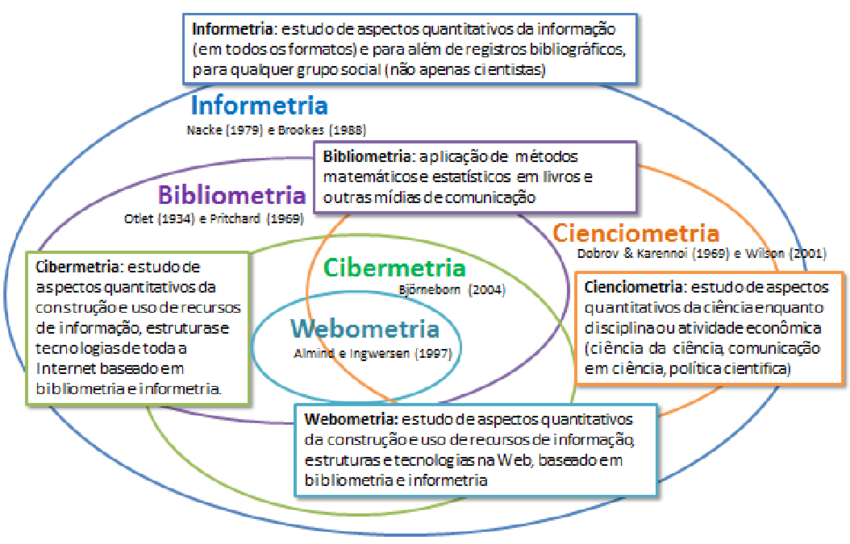
\includegraphics[trim = 0 0 0 0, clip, width=0.6\textwidth]{biblioeconomia.png}
        %\caption{.}
    \end{figure}
%*----------- notes
    \note[item]{Notes can help you to remember important information. Turn on the notes option.}
\end{frame}
%-
%*----------- SLIDE -------------------------------------------------------------
\begin{frame}[t]{Bibliometria}
    \begin{itemize}
        \item É um campo da biblioteconomia e da ciência da informação.
        \item Aplica métodos estatísticos e matemáticos para analisar e construir indicadores sobre a dinâmica e evolução da informação científica e tecnológica.
        \item Medir o impacto das publicações e dos serviços de disseminação da informação.
        \item Identificar autores e instituições mais produtivas.
        \item Todos os estudos que tentam quantificar os processos de comunicação escrita. \cite{pritchard1969statistical}
        \item Avaliar a produção científica. \cite{costa2020ciencia}
        \item Estudar relações entre a ciência e a tecnologia. \cite{maricato2010dinamica}
    \end{itemize}

    \begin{figure}
        
\includegraphics[trim = 0 0 0 0, clip, width=0.7\textwidth]{books-banner.jpeg}
        %\caption{.}
    \end{figure}
   
    % \begin{columns}[t]
    %     \column{.45\textwidth}
    %         detalhar sistemas em subconjuntos\\
    %         listar possíveis modos de falhas\\
    %         analisar cada modo de falha, juntamente com suas possíveis causas e sintomas
    %     \column{.45\textwidth}
    %         estimar os efeitos de cada modo de falhas\\
    %         estimar a criticidade de cada efeito\\
    %         identificar ações para minimizar falhas
    % \end{columns}
%*----------- notes
    \note[item]{Notes can help you to remember important information. Turn on the notes option.}
\end{frame}
%-
%*----------- SLIDE -------------------------------------------------------------
\begin{frame}[t]{Principais autores}
    %\framesubtitle{Lei de Bradford}
    % \begin{figure}
    %     %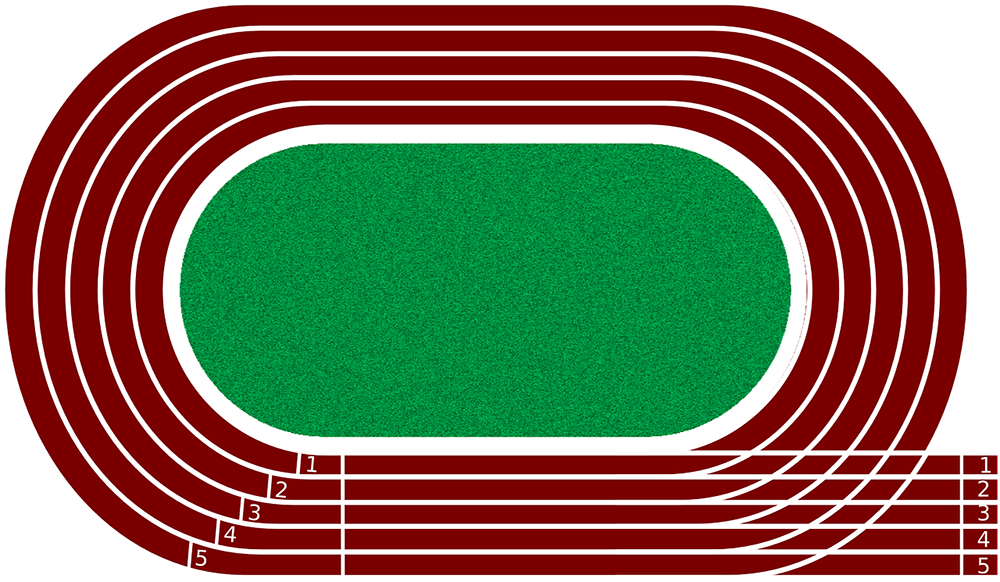
\includegraphics[width=0.7\textwidth]{pista_corrida}
       
    %     \roundpic[xshift=0cm,yshift=0cm]{3cm}{7cm}{pista_corrida}
          
    %     \caption{Formato de um pista de corrida.\cite{agostini2007}}
    % \end{figure}

    \begin{columns}
        %\column{.01\textwidth}
        \column{.33\textwidth}
            \centering
            \roundpic[xshift=0cm,yshift=-0.5cm]{5cm}{7cm}{Samuel_Clemente_Bradford}
            Samuel Clement Bradford\\
            1934
        \column{.33\textwidth}
            \centering
            \roundpic[xshift=0cm,yshift=0cm]{5cm}{7cm}{Alfredo-Lotka}
            Alfred James Lotka\\
            1926
        \column{.33\textwidth}
            \centering
            \roundpic[xshift=0cm,yshift=-1cm]{5cm}{7cm}{George-Zipf}
            George Kingsley Zipf\\
            1940
    \end{columns}

%*----------- notes
    \note[item]{Notes can help you to remember important information. Turn on the notes option.}
\end{frame}
%-
%*----------- SLIDE -------------------------------------------------------------
\begin{frame}[t]{As principais leis bibliométricas}
    \framesubtitle{Lei de Bradford}
    % \begin{figure}
    %     %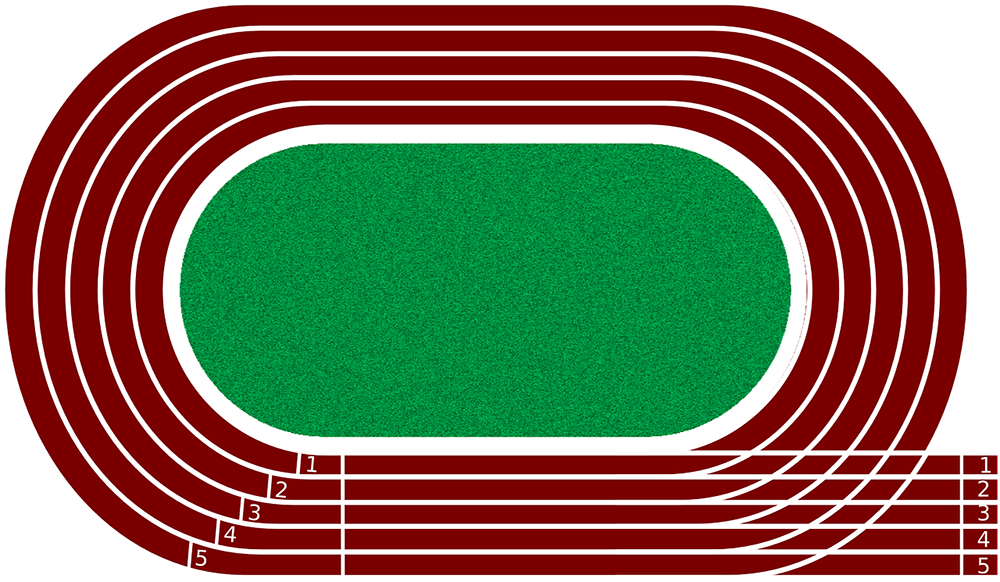
\includegraphics[width=0.7\textwidth]{pista_corrida}
       
    %     \roundpic[xshift=0cm,yshift=0cm]{3cm}{7cm}{pista_corrida}
          
    %     \caption{Formato de um pista de corrida.\cite{agostini2007}}
    % \end{figure}

    \begin{columns}
        \column{.1\textwidth}
        \column{.3\textwidth}

        \begin{figure}
            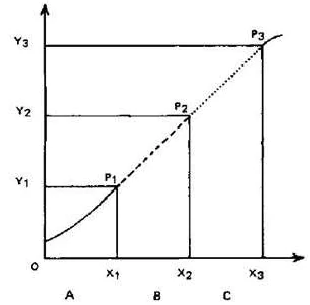
\includegraphics[trim = 0 0 0 0, clip, width=0.7\textwidth]{bradford-2.png}
            %\caption{.}
        \end{figure}

        \centering
        $F(x) = a + b \log x$
        \column{.69\textwidth}
        A lei de Bradford objetiva conhecer o núcleo de periódicos produzidos em determinado tema.\\
        \scriptsize{
            Bradford realiza uma série de estudos que culminam, em 1934, com a formulação da \textbf{lei da dispersão}.\\
            O autor percebe que, numa coleção de periódicos sobre geofísica, existe sempre um núcleo menor de periódicos relacionados de maneira estreita, sendo que o número de perióidocs em cad zona aumenta, enquanto a produtividade diminui.\\
            Analisando 326 períodicos, ele descobriu que 9 periódicos continham 429 artigos, 59 continham 499 e 258 continham 404 artigos.
        }
    \end{columns}

    \vspace*{0.2cm}
    \begin{itemize}
        \item Medir produtividade dos periódicos
        \item Estabelecer núcleo e as áreas de dispersão 
        \item Permite fazer a estimativa do grau de relevância das revistas de conhecimentos
    \end{itemize}
%*----------- notes
    \note[item]{Notes can help you to remember important information. Turn on the notes option.}
\end{frame}
%-
%*----------- SLIDE -------------------------------------------------------------
\begin{frame}[t]{As principais leis bibliométricas}
    \framesubtitle{Lei de Lotka}
    % \begin{figure}
    %     %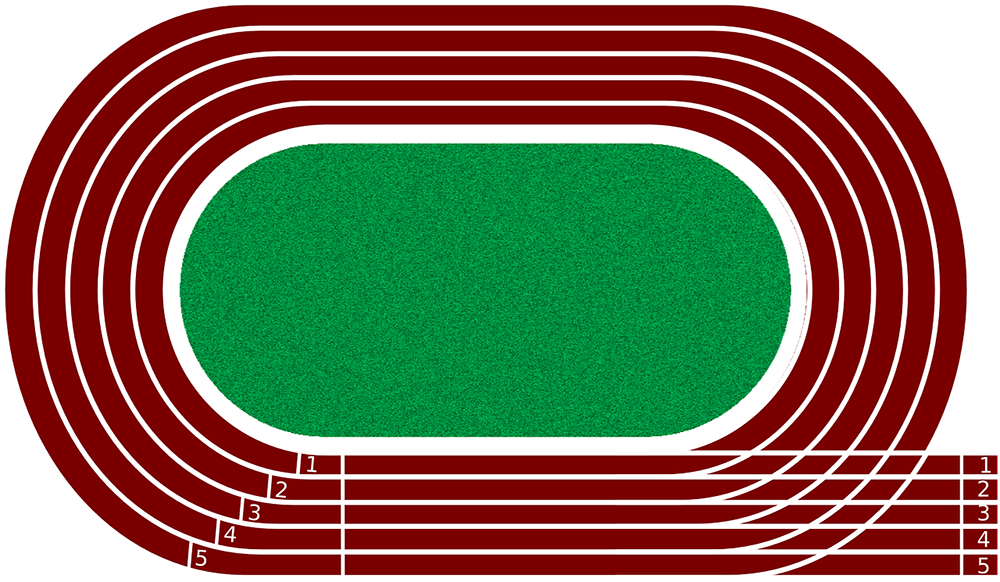
\includegraphics[width=0.7\textwidth]{pista_corrida}
       
    %     \roundpic[xshift=0cm,yshift=0cm]{3cm}{7cm}{pista_corrida}
          
    %     \caption{Formato de um pista de corrida.\cite{agostini2007}}
    % \end{figure}

    \begin{columns}
        \column{.01\textwidth}
        \column{.5\textwidth}

        \begin{figure}
            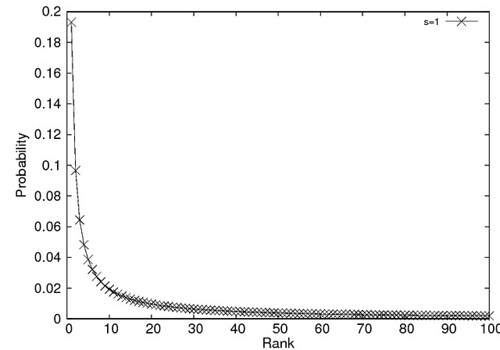
\includegraphics[trim = 0 0 0 0, clip, width=0.6\textwidth]{lotka}
            %\caption{.}
        \end{figure}

        \centering
        $Y = \frac{C}{X^n}$\\
        $Y$ \scriptsize{é a frequência relativa de autores com $X$ publicações.}\\
        $C$ \scriptsize{é a constante que depende da área $X$ é o número de publicações.}

        \column{.49\textwidth}
        A lei de Lotka visa definir as maiores contribuições de pesquisadores em determinadas áreas do conhecimento.\\
        %\scriptsize{
            Lotka descobriu que uma larga proporção da literatura científica é produzida por um pequeno número de autores, e um grande número de pequenos produtores se iguala, em produção, ao reduzido número de grandes produtores.
        %}
    \end{columns}

    \vspace*{0.2cm}

%*----------- notes
    \note[item]{Notes can help you to remember important information. Turn on the notes option.}
\end{frame}
%-
%*----------- SLIDE -------------------------------------------------------------
\begin{frame}[t]{As principais leis bibliométricas}
    \framesubtitle{Lei de Zipf}
    % \begin{figure}
    %     %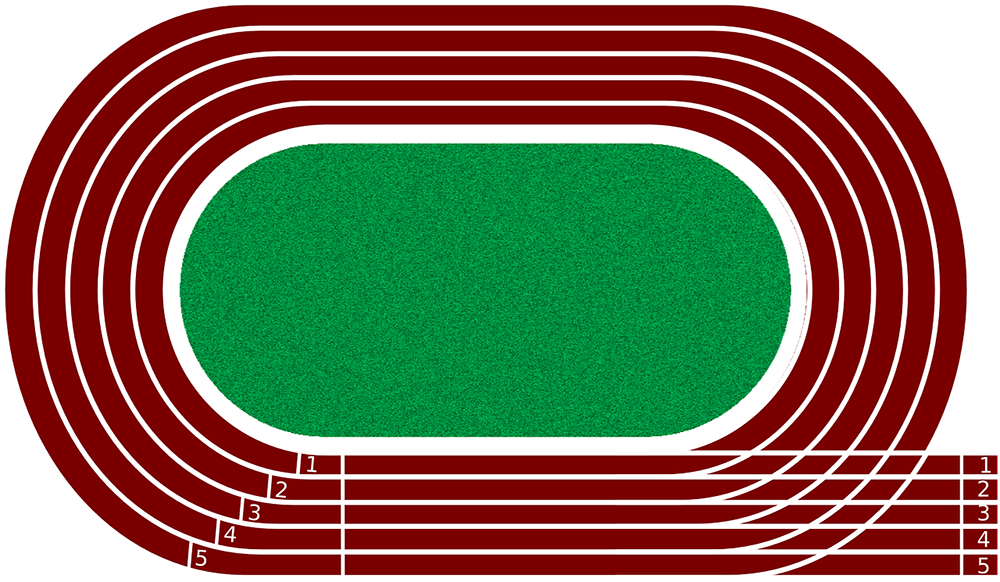
\includegraphics[width=0.7\textwidth]{pista_corrida}
       
    %     \roundpic[xshift=0cm,yshift=0cm]{3cm}{7cm}{pista_corrida}
          
    %     \caption{Formato de um pista de corrida.\cite{agostini2007}}
    % \end{figure}

    \begin{columns}
        \column{.01\textwidth}
        \column{.5\textwidth}

        \begin{figure}
            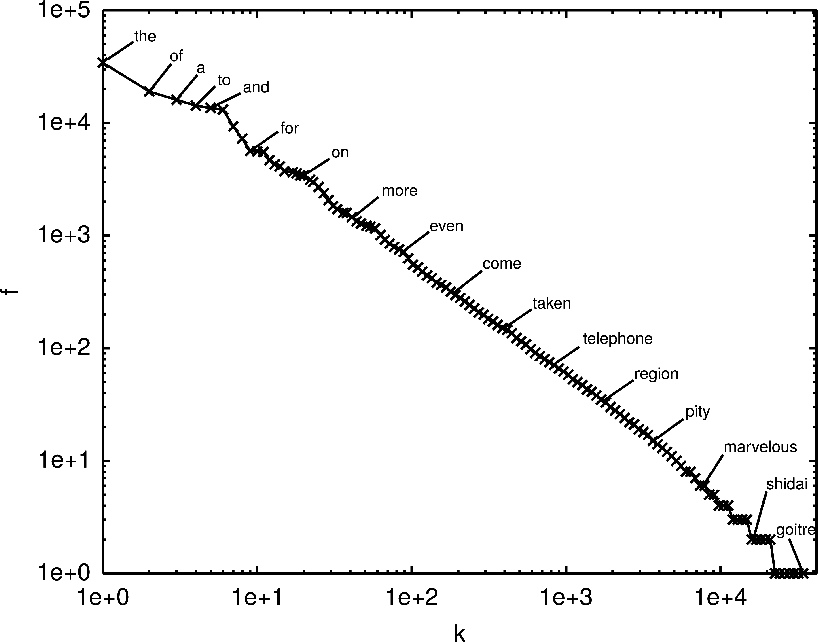
\includegraphics[trim = 0 0 0 0, clip, width=0.5\textwidth]{Figura-1-Lei-de-Zipf-no-Ingles-escrito-dados-do-OANC-Rank-k-versus-frequencia-de.png}
            %\caption{.}
        \end{figure}

        \centering
        $f(n) = \frac{K}{n}$\\
        $f(n)$ \scriptsize{é a frequência de ocorrência de uma palavra}\\
        $n$ \scriptsize{é a ordem de frequência}
        $K$ \scriptsize{é a constante}\\

        \column{.49\textwidth}
        A lei de Zipf pontua a frequência com que certas palavras aparecem nos textos científicos de maneira a definir sua representatividade neste contexto.\\
        \scriptsize{
            Diante desta visão, Zipf formulou o \textbf{princípio do menor esforço}: existe uma economia do uso de palavras, e se a tendência é usar o mínimo significa que elas não vão se dispersar, pelo contrário, uma mesma palavra vais ser usada muitas vezes; as palavras mais usadas indicam o assunto do documento.
        }
    \end{columns}

    \vspace*{0.2cm}
    \begin{itemize}
        \item Trata e mede a frequência de ocorrência de palavras em vários textos.
        \item As palavras mais usadas indicam o assunto.
    \end{itemize}
%*----------- notes
    \note[item]{Notes can help you to remember important information. Turn on the notes option.}
\end{frame}
%-
%*----------- SLIDE -------------------------------------------------------------
\begin{frame}[t]{O fator de impacto}
    %\transboxin[duration=1,direction=30]
    \large{Medida que reflete o número médio de citações de artigos científicos publicados.}\\

    \vspace*{0.2cm}
	Tem como objetivo avaliar a importância de um dado periódico em sua área.

    \begin{figure}
        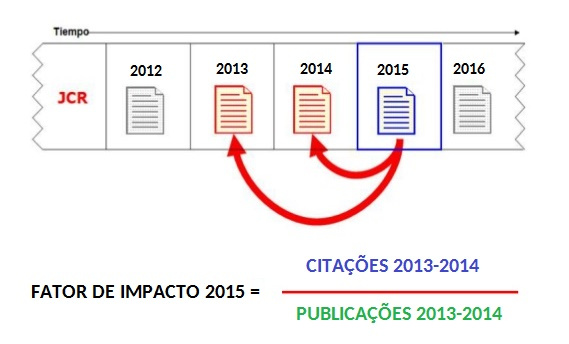
\includegraphics[trim = 0 0 0 0, clip, width=0.6\textwidth]{fi.jpg}
        %\caption{.}
    \end{figure}
%*----------- notes
    \note[item]{Notes can help you to remember important information. Turn on the notes option.}
\end{frame}
%-
%*----------- SLIDE -------------------------------------------------------------
\begin{frame}{Principais estudos da Bibliometria}
    % \begin{table}[ht!]
    %     \centering
    %         \caption{PERCENTUAL DE CONCLUSÃO POR EQUIPE}
    %         \begin{tabular}{|l|c|c|c|c|} \hline
    %             \textbf{EQUIPE}&\textbf{04/05}&\textbf{11/05}&\textbf{18/05}&\textbf{25/05}\\ \hline
    %             RAJA & 17\% &32\% & &  \\ \hline
    %             BORG & 0\% &41\% & &  \\ \hline
    %             TIMON-HM & 5\% &47\% & &  \\ \hline
    %         \end{tabular}
    % \end{table}

	\begin{table}[ht!]
		%\scalefont{0.7}
        \resizebox{0.9\textwidth}{!}{
		\begin{tabular}{|l|c|l|}
            \hline
            \multicolumn{1}{|c|}{\textbf{Leis e Princípios}} & \textbf{Foco de Estudo} & \multicolumn{1}{c|}{\textbf{Principais Aplicações}}                                                                         \\ \hline
            Lei de Bradford                                  & periódicos               & \begin{tabular}[c]{@{}l@{}}estimar o grau de relevância de periódicos\end{tabular}         \\ \hline
            Lei de Lotka                                     & autores                  & \begin{tabular}[c]{@{}l@{}}estimar o grau de relevância de autores\end{tabular}            \\ \hline
            Leis de Zipf                                     & palavras                 & \begin{tabular}[c]{@{}l@{}}indexação automática de artigos científicos\\ e tecnológicos\end{tabular}                        \\ \hline
            Fator de Impacto               & citações                 & \begin{tabular}[c]{@{}l@{}}estimar o grau de relevância de artigos, \\ cientistas e periódicos científicos\end{tabular} \\ \hline
            Acoplamento Bibliográfico                        & citações                 & \begin{tabular}[c]{@{}l@{}}estimar o grau de ligação de dois ou mais \\ artigos\end{tabular}                                \\ \hline
            Co-citação                                       & citações                 & \begin{tabular}[c]{@{}l@{}}estimar o grau de ligação de dois ou mais \\ artigos\end{tabular}                                \\ \hline
            Obsolescência da Literatura                      & citações                 & \begin{tabular}[c]{@{}l@{}}estimar o declínio da literatura de \\ determinada área do conhecimento\end{tabular}             \\ \hline
            Vida-média                                       & citações                 & \begin{tabular}[c]{@{}l@{}}estimar a vida-média de uma unidade da\\  literatura de dada área do conhecimento\end{tabular}   \\ \hline
		\end{tabular}
        }
	\end{table}

%*----------- notes
\note[item]{Notes can help you to remember important information. Turn on the notes option.}
\end{frame}
%-
%*----------- SLIDE -------------------------------------------------------------
\begin{frame}[c]{}

    \centering
    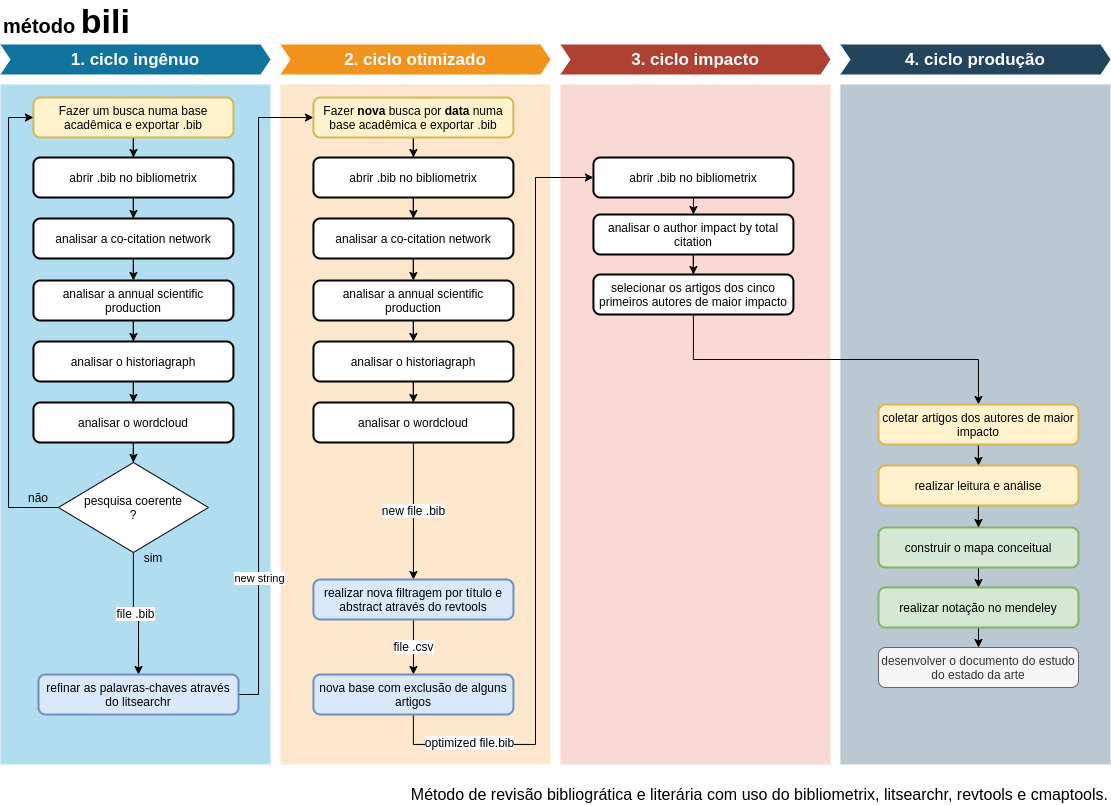
\includegraphics[width=.85\textwidth, trim= 0 30 0 0, clip]{revisão bibliogrática Diagram.png}
    
        
    % \begin{tikzpicture}[remember picture,overlay]
    %     \draw[red,very thick] (cmark) circle[x radius=8mm,y radius=4mm]; 
    % \end{tikzpicture}
%*----------- notes
    \note[item]{Notes can help you to remember important information. Turn on the notes option.}
\end{frame}
%-
%*----------- SLIDE -------------------------------------------------------------
\begin{frame}[t]{Ciclo Ingênuo}
    
    \begin{columns}
        \column{.01\textwidth}
        \column{.5\textwidth}
            \centering
            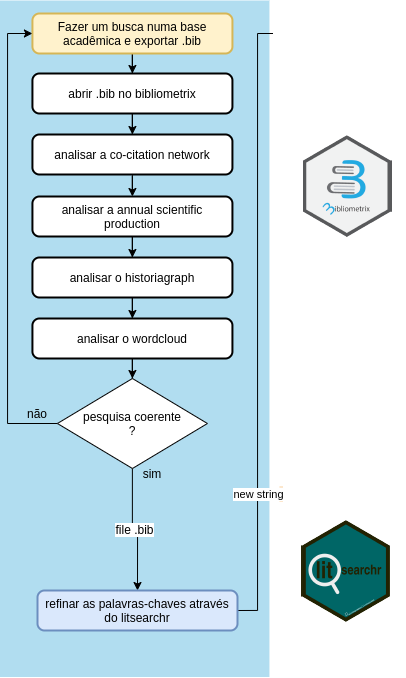
\includegraphics[width=.55\textwidth, trim= 0 0 0 0, clip]{ciclo1.png}
        \column{.6\textwidth}
            \centering
            Fazer uma busca numa base acadêmica e exportar no formato \emph{.bib}\\

            \vspace*{0.2cm}
            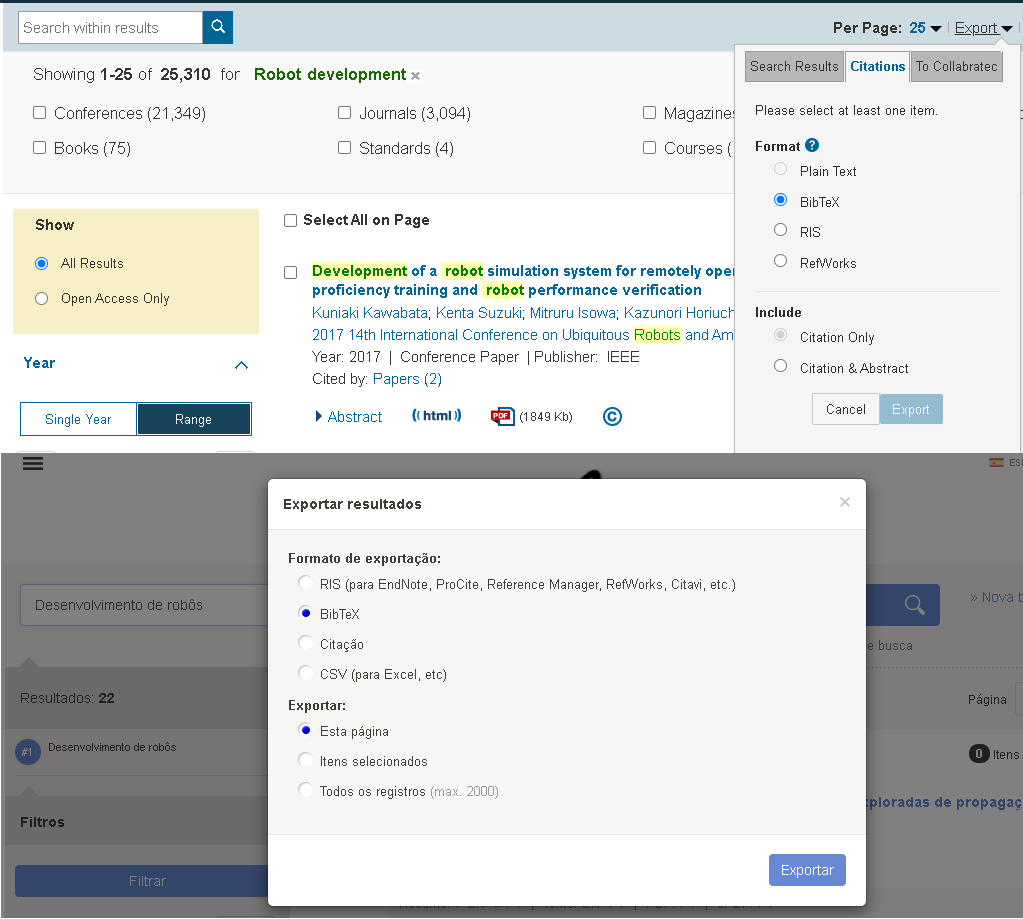
\includegraphics[width=.55\textwidth, trim= 0 0 0 0, clip]{bases.png}
    \end{columns}

%*----------- notes
    \note[item]{Notes can help you to remember important information. Turn on the notes option.}
\end{frame}
%-
%*----------- SLIDE -------------------------------------------------------------
\begin{frame}[t]{Ciclo Ingênuo}
    
    % \begin{columns}
    %     \column{.01\textwidth}
    %     \column{.5\textwidth}
    %         \centering
    %         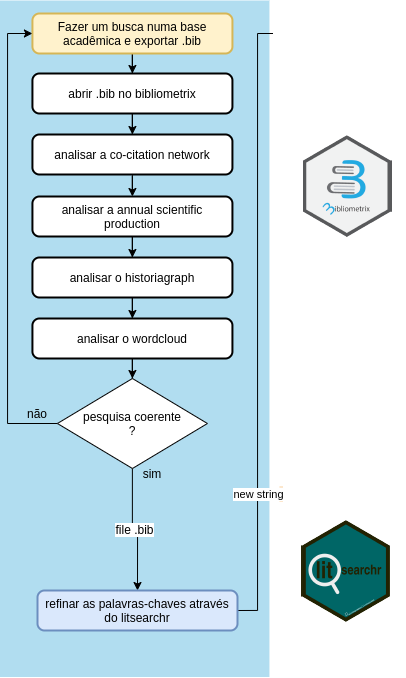
\includegraphics[width=.55\textwidth, trim= 0 0 0 0, clip]{ciclo1.png}
    %     \column{.6\textwidth}
    %         \centering
    %         Fazer uma busca numa base acadêmica e exportar no formato \emph{.bib}\\

    %         \vspace*{0.2cm}
    %         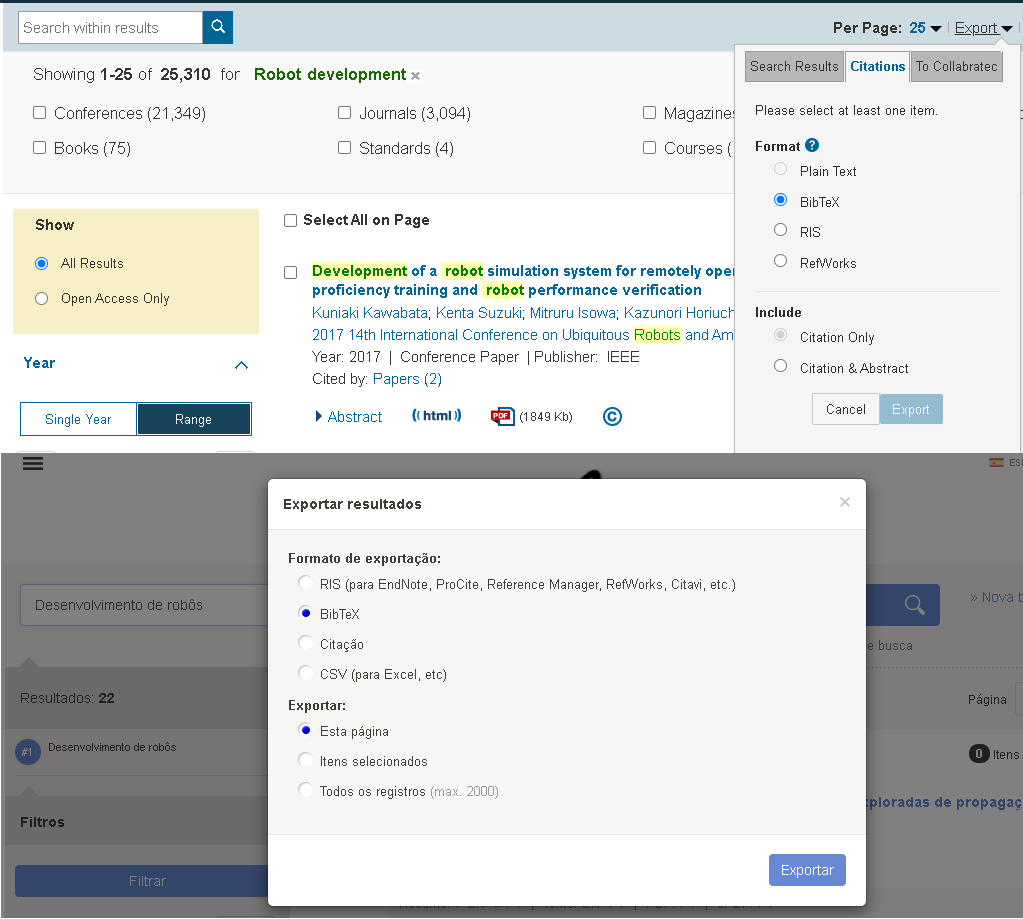
\includegraphics[width=.55\textwidth, trim= 0 0 0 0, clip]{bases.png}
    % \end{columns}
    \begin{tcolorbox}[colback=gcolor!5!white,colframe=gcolor!75!black,title=String]
        (("underwater manipulator" OR "underwater vehicle manipulator system") AND ("underwater robot" OR "underwater vehicle" OR "autonomous underwater") AND ("disturbance observer"))
    \end{tcolorbox}

    \centering
    \centerline{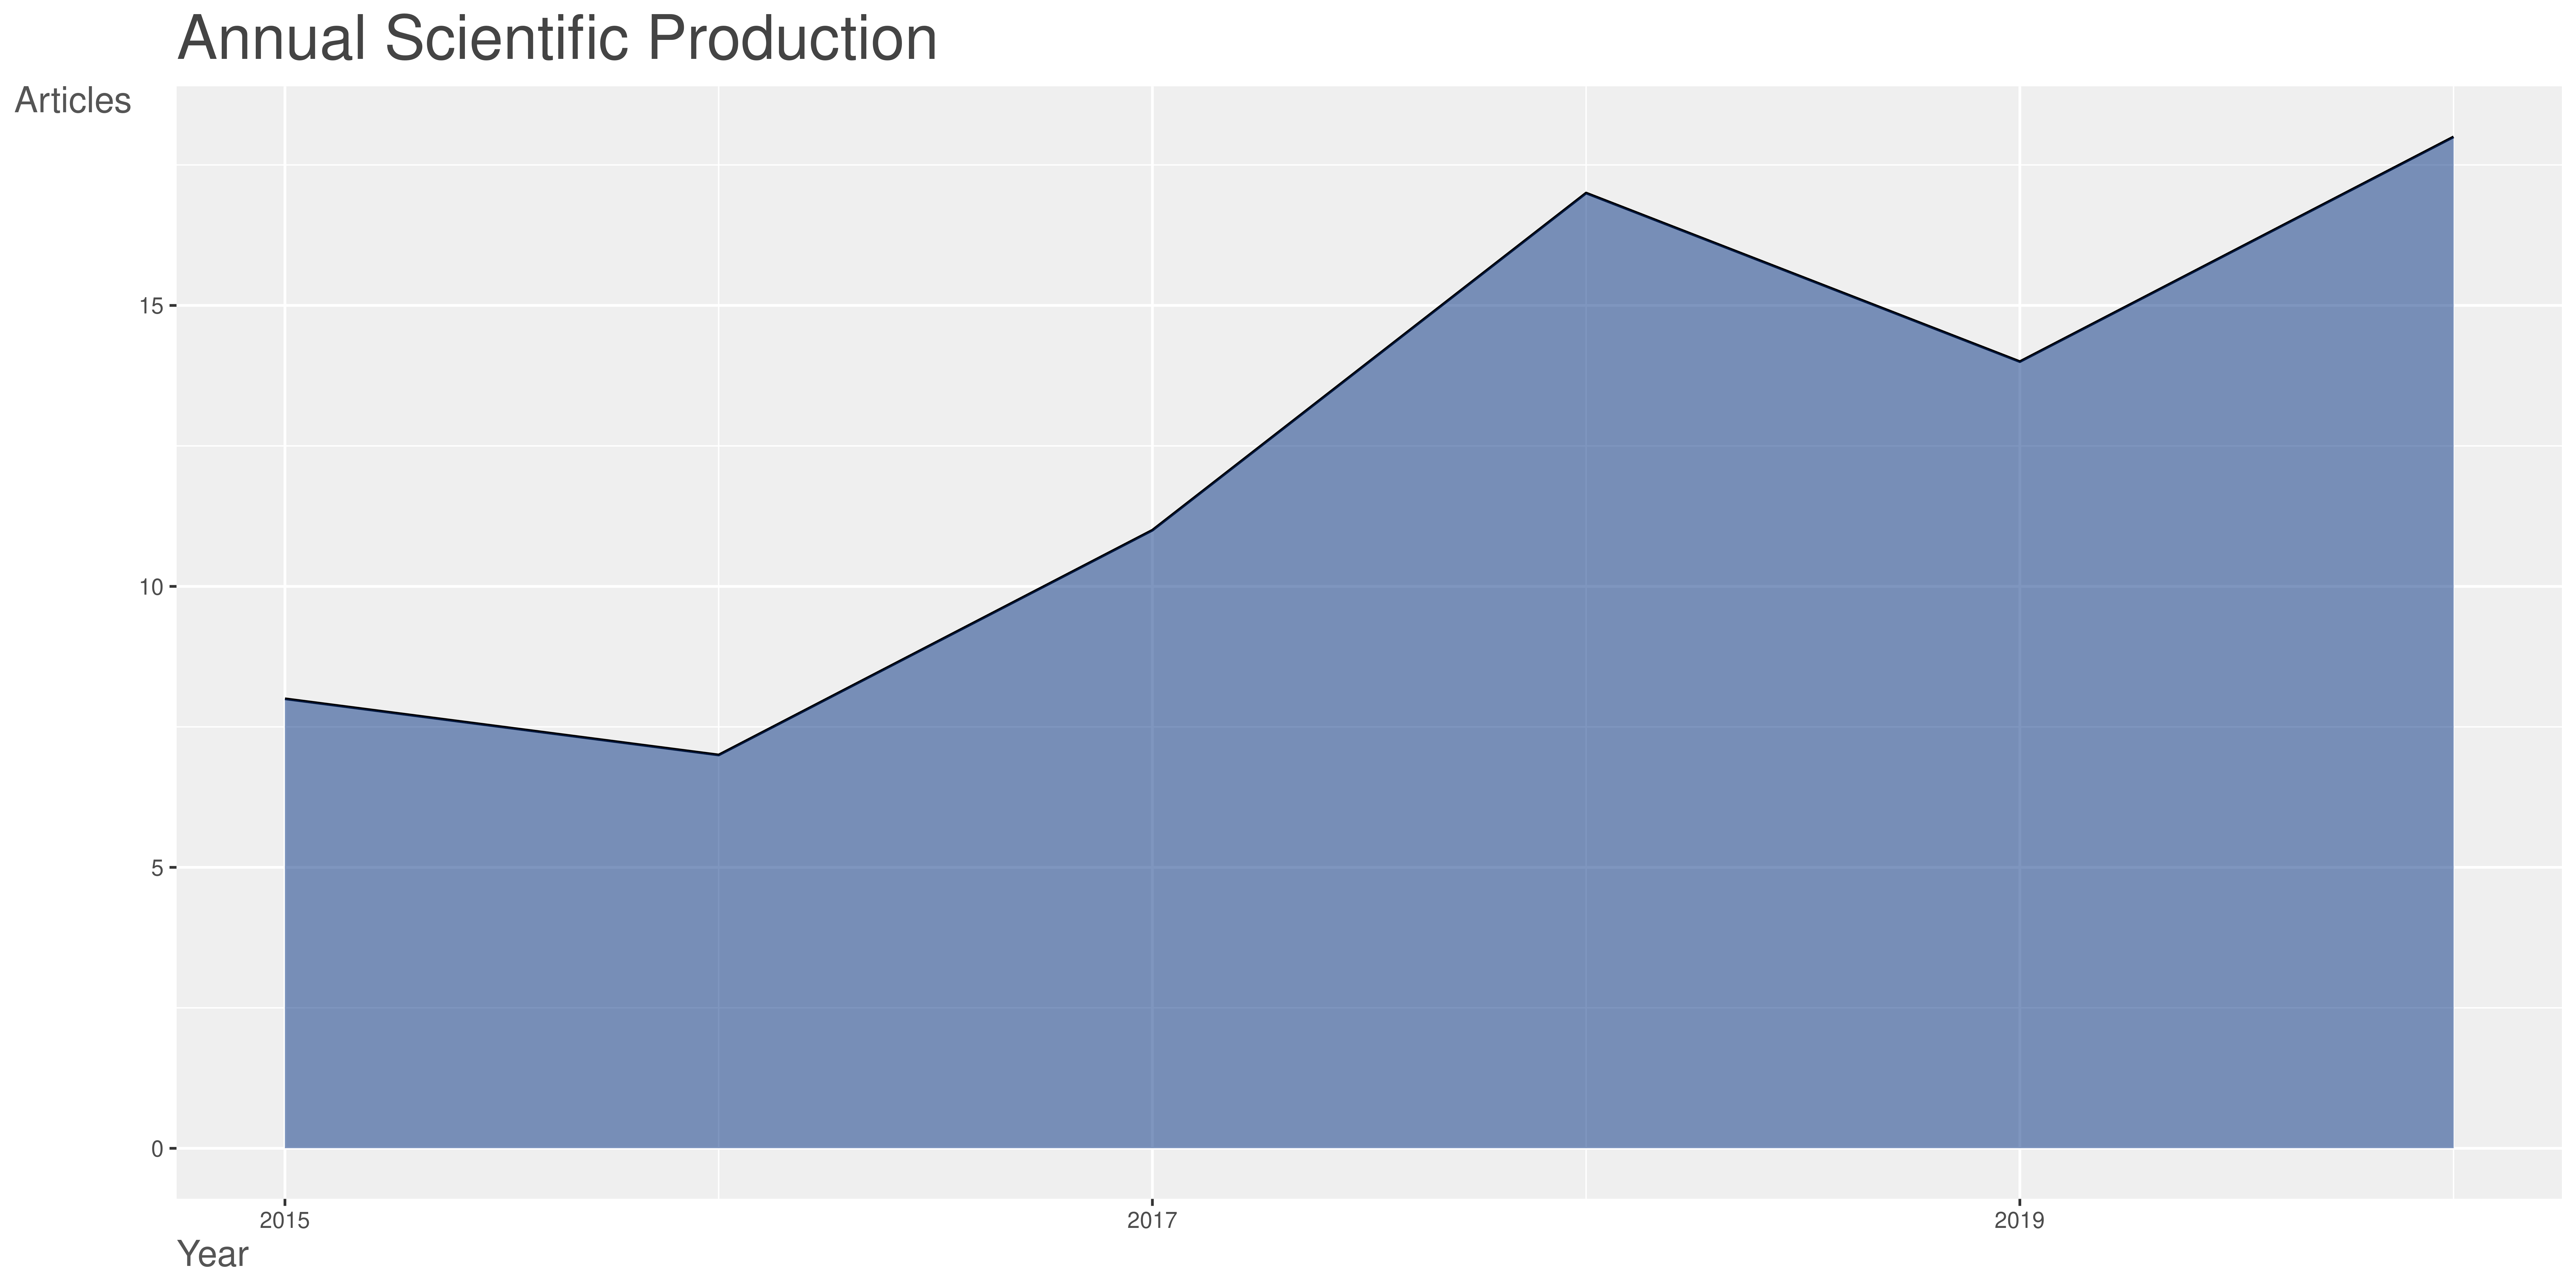
\includegraphics[trim = 0 0 0 0, clip, width=0.5\textwidth]{AnnualScientificProduction-2021-04-28.png}}

%*----------- notes
    \note[item]{Notes can help you to remember important information. Turn on the notes option.}
\end{frame}
%-
%*----------- SLIDE -------------------------------------------------------------
\begin{frame}[t]{Ciclo Ingênuo}
    
    % \begin{columns}
    %     \column{.01\textwidth}
    %     \column{.5\textwidth}
    %         \centering
    %         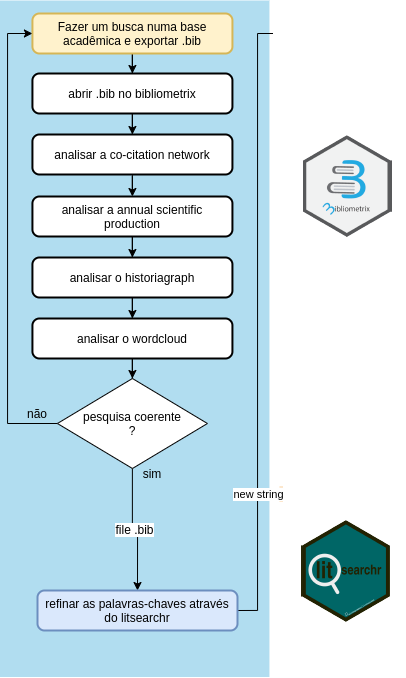
\includegraphics[width=.55\textwidth, trim= 0 0 0 0, clip]{ciclo1.png}
    %     \column{.6\textwidth}
    %         \centering
    %         Fazer uma busca numa base acadêmica e exportar no formato \emph{.bib}\\

    %         \vspace*{0.2cm}
    %         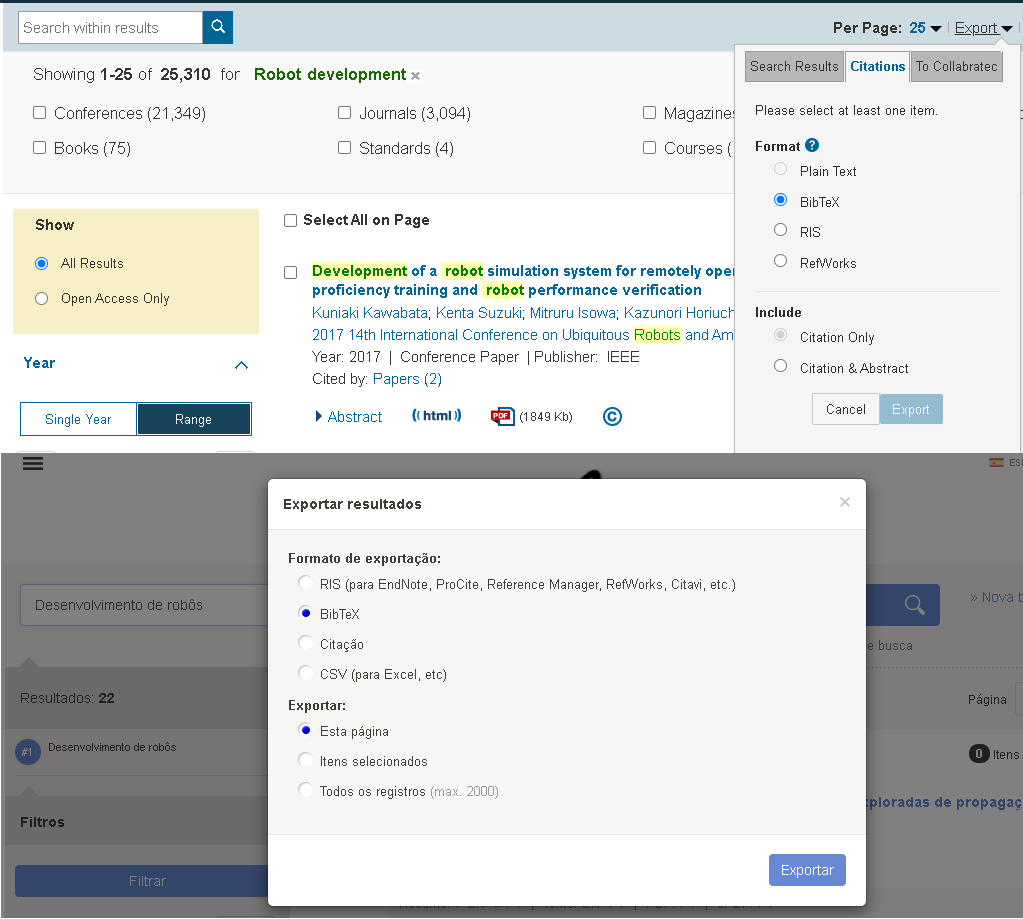
\includegraphics[width=.55\textwidth, trim= 0 0 0 0, clip]{bases.png}
    % \end{columns}
    \centering
    \centerline{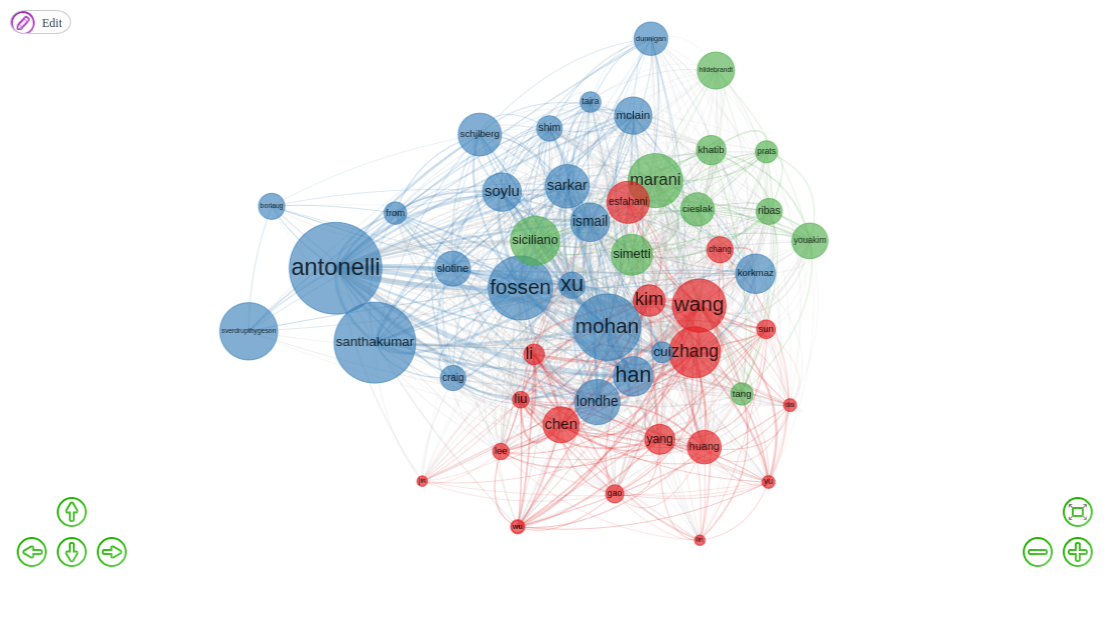
\includegraphics[trim = 0 0 0 0, clip, width=.9\textwidth]{network (3).png}}

%*----------- notes
    \note[item]{Notes can help you to remember important information. Turn on the notes option.}
\end{frame}
%-
%*----------- SLIDE -------------------------------------------------------------
\begin{frame}[t]{uma nova string}
    
    \centering
    \centerline{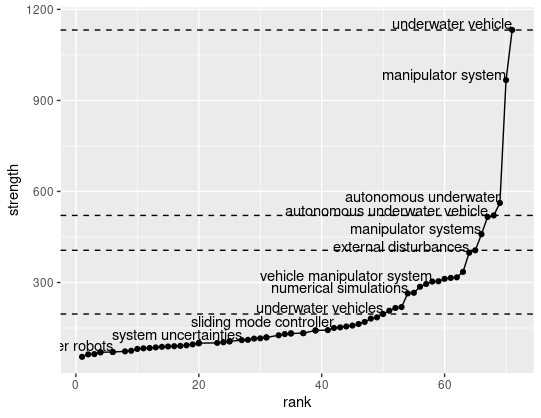
\includegraphics[trim = 0 0 0 0, clip, width=0.35\textwidth]{Rplot03.png}}

    \centering
    \centerline{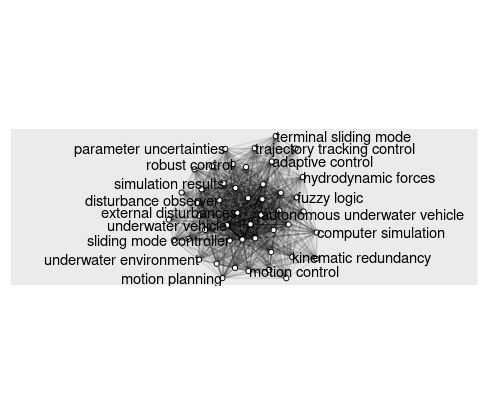
\includegraphics[trim = 0 70 0 80, clip, width=0.5\textwidth]{Rplot04.png}}


%*----------- notes
    \note[item]{Notes can help you to remember important information. Turn on the notes option.}
\end{frame}
%-
%*----------- SLIDE -------------------------------------------------------------
\begin{frame}[c]{uma nova string}
    
    \begin{tcolorbox}[colback=gcolor!5!white,colframe=gcolor!75!black,title=String Refinada]
        (("manipulator system" OR "underwater manipulator" OR "vehicle manipulator system" OR "underwater vehicle manipulator system") AND ("underwater manipulator" OR "underwater robot" OR "underwater vehicle" OR "autonomous underwater") AND ("disturbance observer" OR "external disturbances" OR "motion planning" OR "trajectory tracking" OR "sliding mode control"))
    \end{tcolorbox}

    
%*----------- notes
    \note[item]{Notes can help you to remember important information. Turn on the notes option.}
\end{frame}
%-
%*----------- SLIDE -------------------------------------------------------------
\begin{frame}[t]{Ciclo Otimizado}
    
    \begin{columns}
        \column{.01\textwidth}
        \column{.5\textwidth}
            \centering
            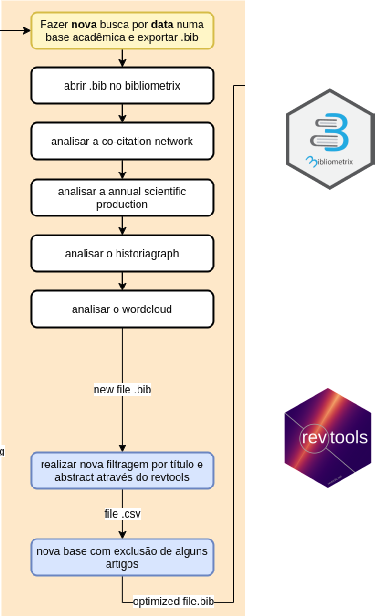
\includegraphics[width=.55\textwidth, trim= 0 0 0 0, clip]{ciclo2.png}
        \column{.6\textwidth}
            \centering
            Testar a nova \emph{string}, e exportar os dados otimizado no formato \emph{.bib}\\

            \vspace*{0.2cm}
            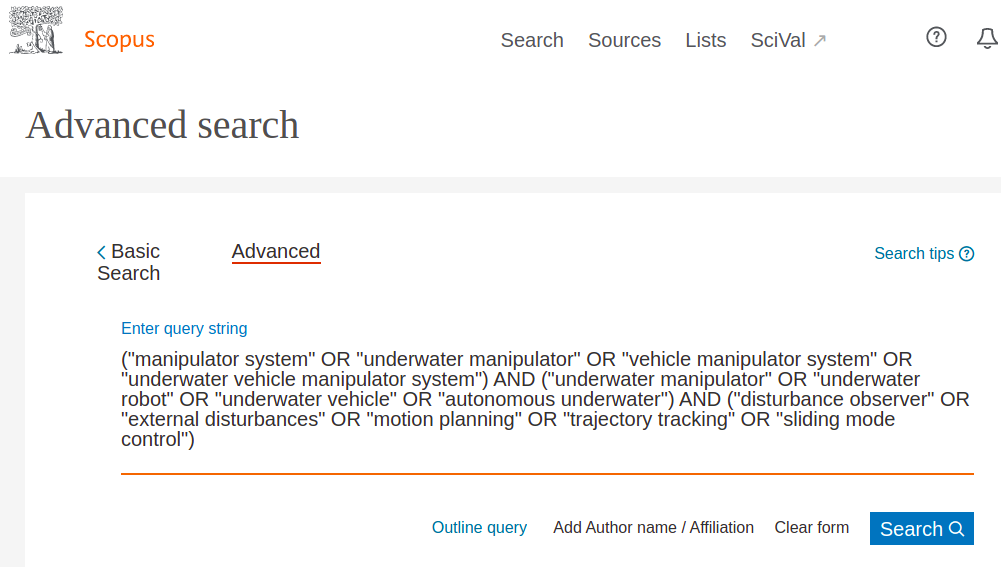
\includegraphics[width=.85\textwidth, trim= 0 0 0 0, clip]{novabusca.png}
    \end{columns}

%*----------- notes
    \note[item]{Notes can help you to remember important information. Turn on the notes option.}
\end{frame}
%-
%*----------- SLIDE -------------------------------------------------------------
\begin{frame}[c]{Ciclo Otimizado}
    
    \begin{columns}
        \column{.01\textwidth}
        \column{.5\textwidth}
            \centering
            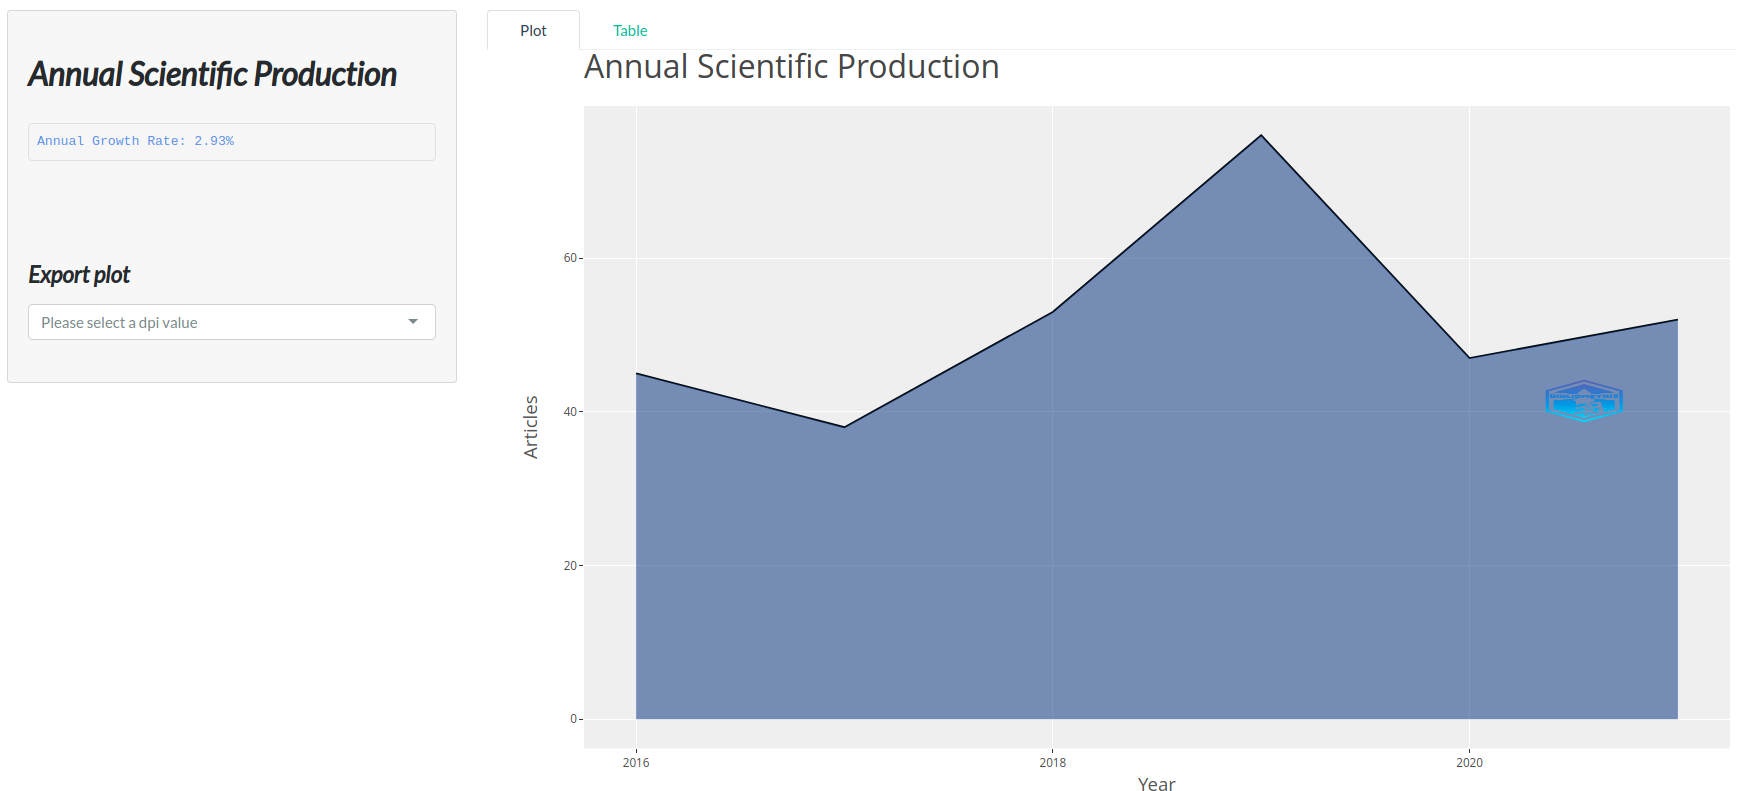
\includegraphics[width=1\textwidth, trim= 500 0 0 0, clip]{turbot1.png}
        \column{.5\textwidth}
            \centering
            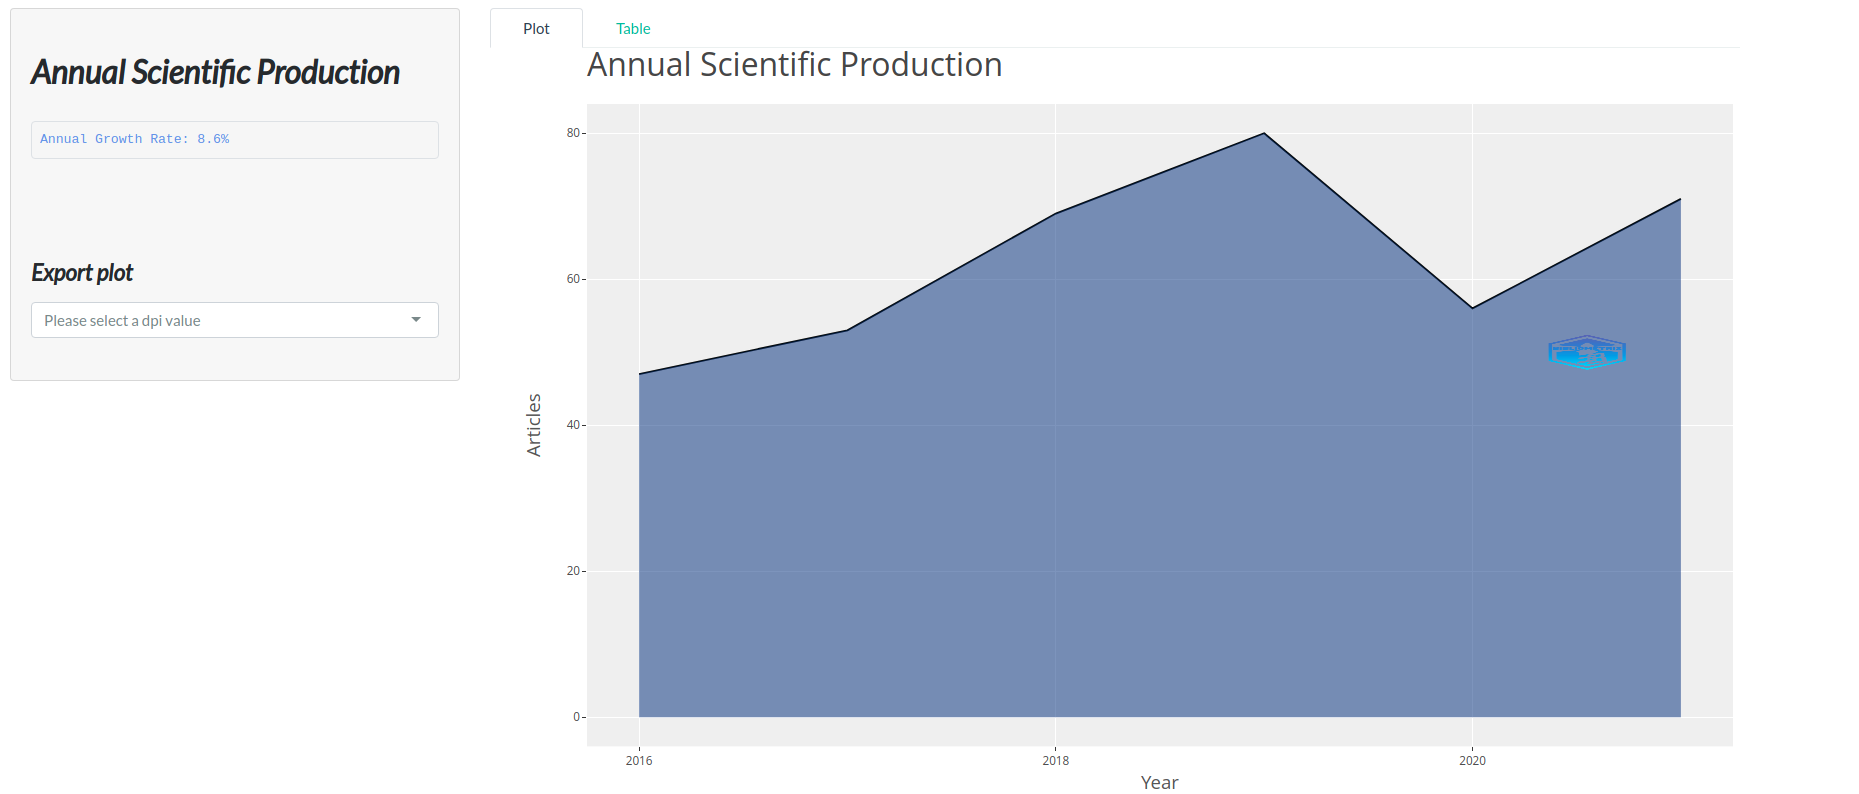
\includegraphics[width=1\textwidth, trim= 500 0 100 0, clip]{turbot2.png}

    \end{columns}

%*----------- notes
    \note[item]{Notes can help you to remember important information. Turn on the notes option.}
\end{frame}
%-
%*----------- SLIDE -------------------------------------------------------------
\begin{frame}[c]{Ciclo Otimizado}
    
    \begin{columns}
        \column{.01\textwidth}
        \column{.5\textwidth}
            \centering
            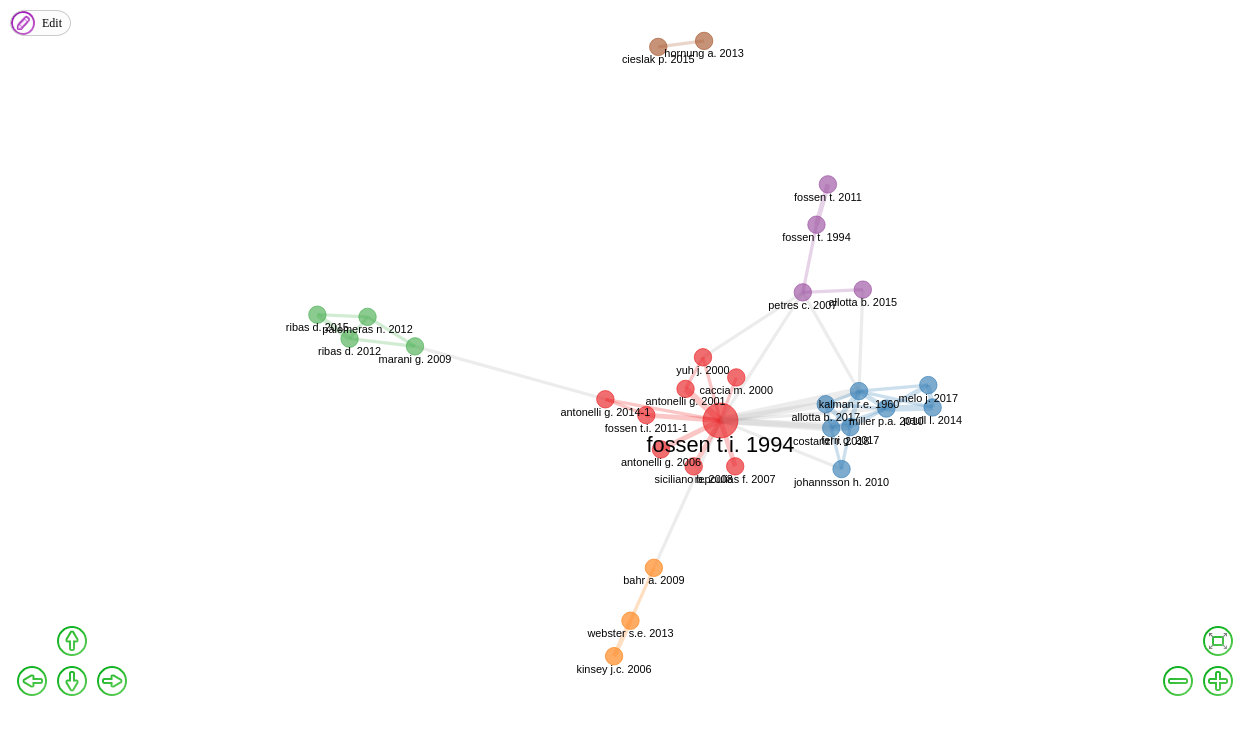
\includegraphics[width=1\textwidth, trim= 200 0 200 0, clip]{turbot3.png}
        \column{.5\textwidth}
            \centering
            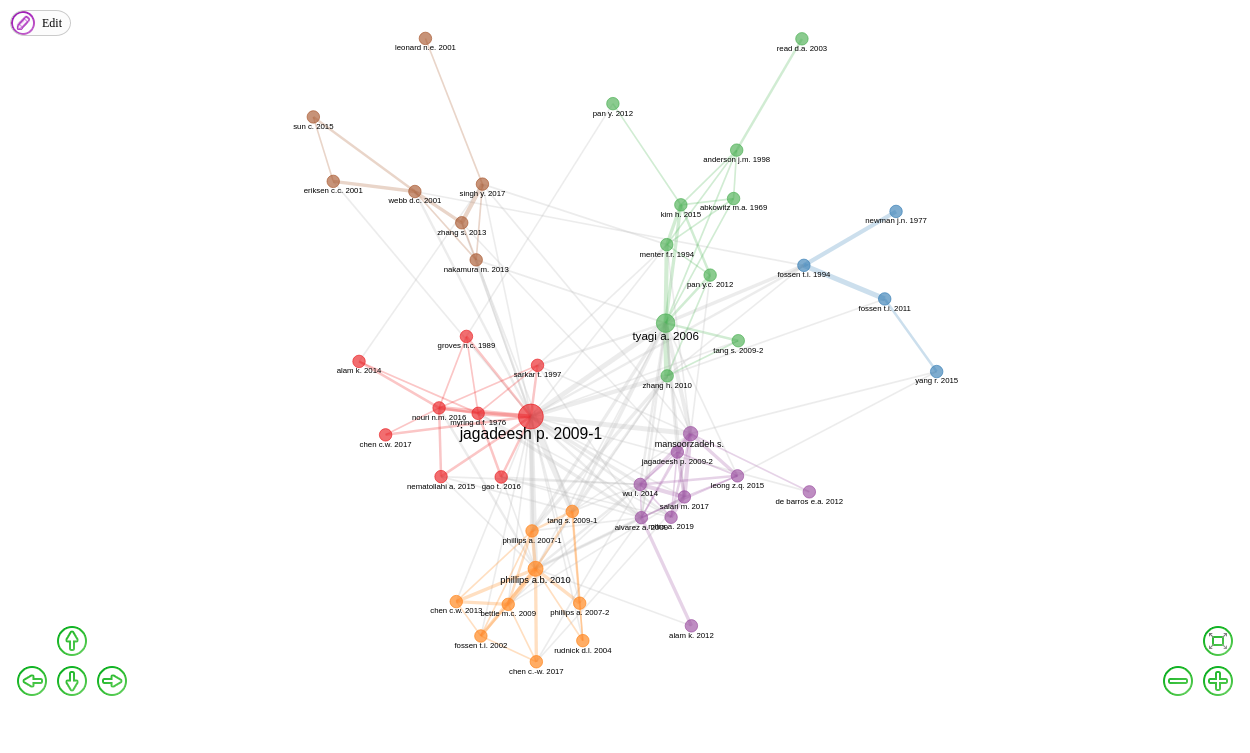
\includegraphics[width=1\textwidth, trim= 200 0 200 0, clip]{turbot4.png}

    \end{columns}

%*----------- notes
    \note[item]{Notes can help you to remember important information. Turn on the notes option.}
\end{frame}
%-
%*----------- SLIDE -------------------------------------------------------------
\begin{frame}[c]{Ciclo Otimizado}
    
    \begin{columns}
        \column{.01\textwidth}
        \column{.5\textwidth}
            \centering
            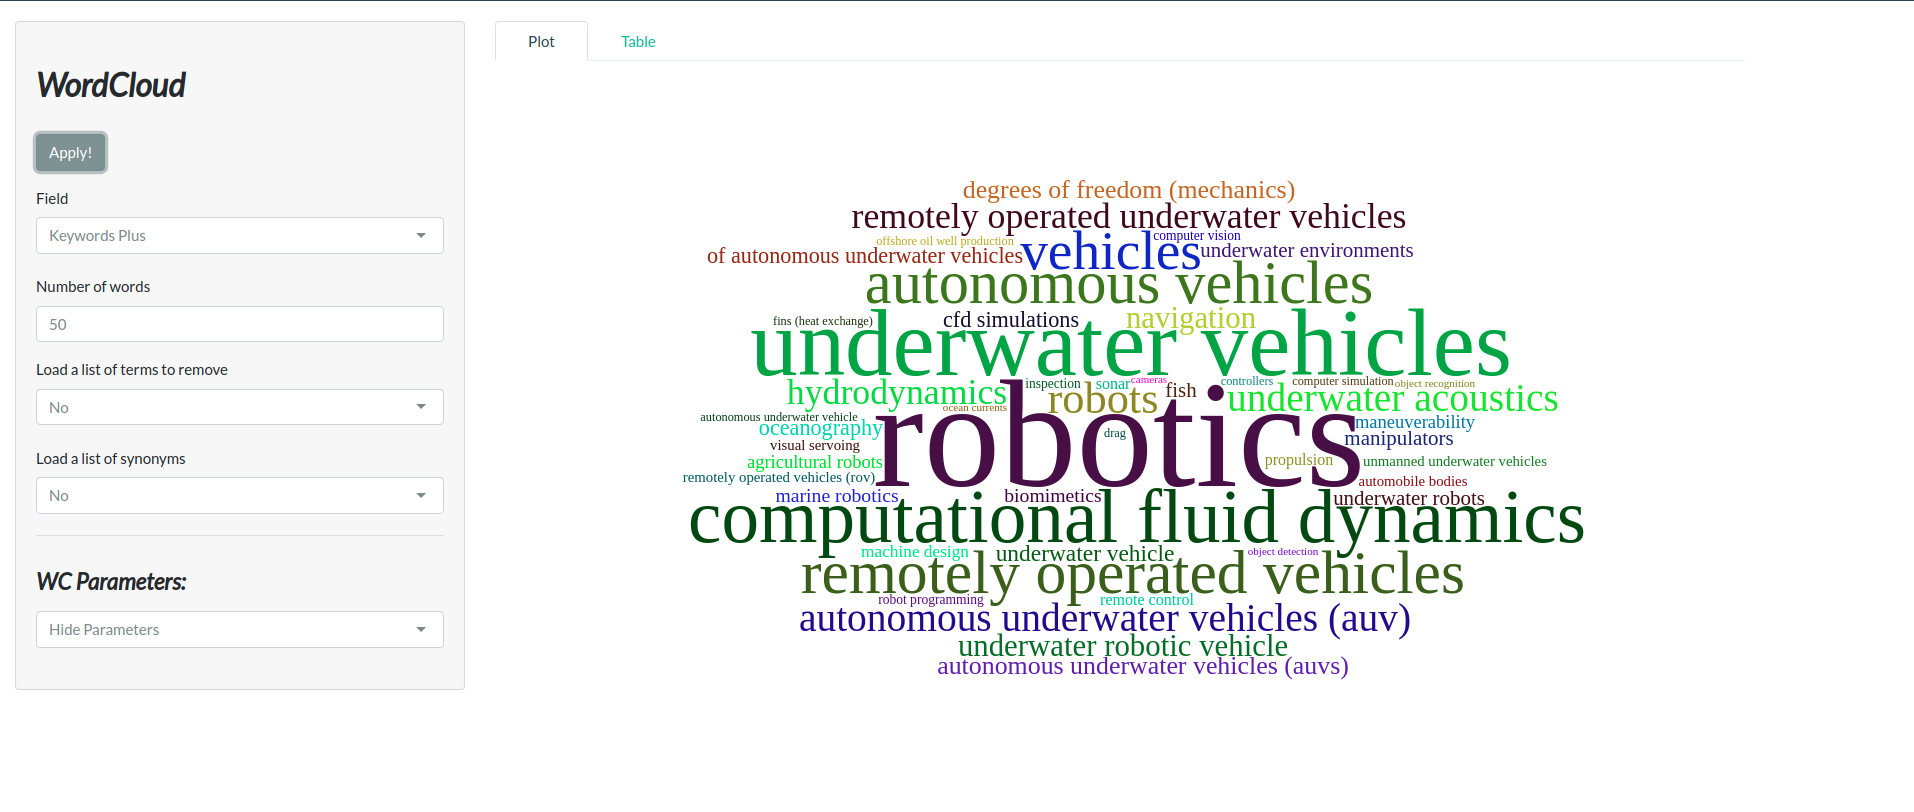
\includegraphics[width=1\textwidth, trim= 600 0 200 0, clip]{turbot5.png}
        \column{.5\textwidth}
            \centering
            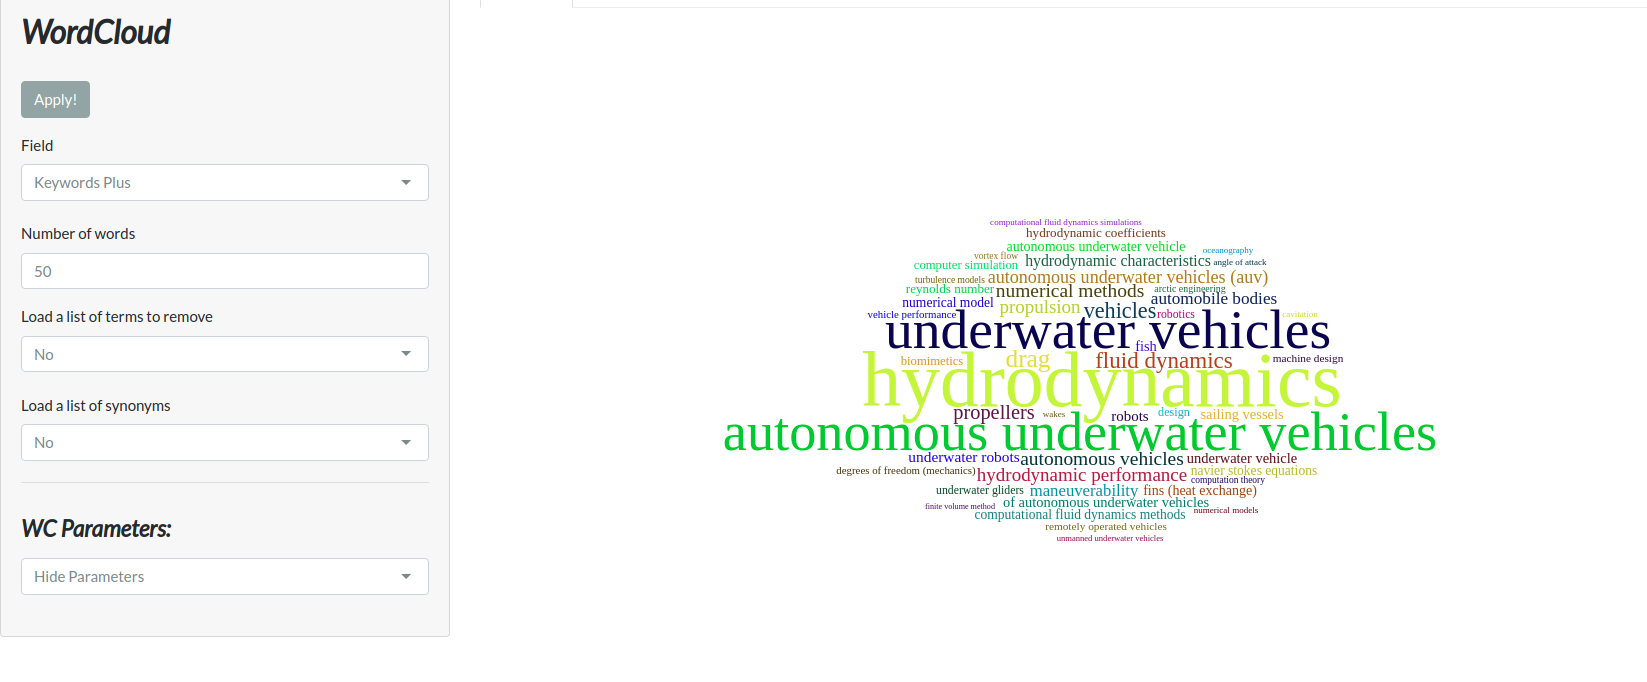
\includegraphics[width=1\textwidth, trim= 700 50 200 100, clip]{turbot6.png}

    \end{columns}

%*----------- notes
    \note[item]{Notes can help you to remember important information. Turn on the notes option.}
\end{frame}
%-
%*----------- SLIDE -------------------------------------------------------------
\begin{frame}[c]{Ciclo Otimizado}
    \framesubtitle{aplicando o RevTools}
    \begin{columns}
        \column{.01\textwidth}
        \column{.5\textwidth}
            \centering
            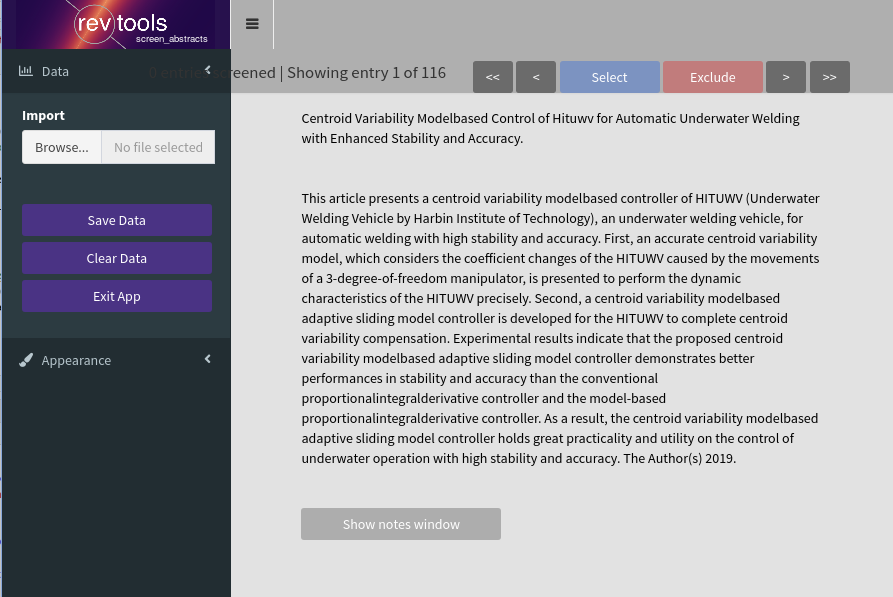
\includegraphics[width=.95\textwidth, trim= 0 0 0 0, clip]{revtools.png}
        \column{.5\textwidth}
    
            O \emph{RevTools} é um pacote do R utilizado para apoiar os pesquisadores que trabalham em projetos de síntese de evidências. \\
            Propicia a visualização baseada em padrões bibliográficos.\\
            Neste método, ele irá promover a exclusão dos artigos que não tem referência com o devido estudo.

    \end{columns}

%*----------- notes
    \note[item]{Notes can help you to remember important information. Turn on the notes option.}
\end{frame}
%-
%*----------- SLIDE -------------------------------------------------------------
\begin{frame}[c]{Ciclo Impacto}
    \begin{columns}
        \column{.01\textwidth}
        \column{.5\textwidth}
            \centering
            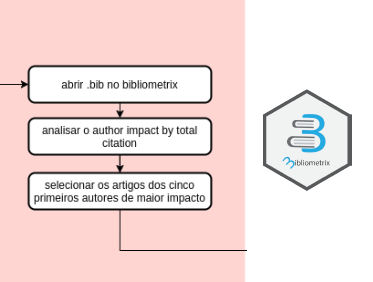
\includegraphics[width=.95\textwidth, trim= 0 0 0 0, clip]{ciclo3.png}
        \column{.5\textwidth}
            Alguns pontos importantes nesta fase:
            \begin{itemize}
                \item Analisar o impacto do autor.
                \item Analisar o impacto do autor por total de citações.
                \item Selecionar os artigos principais dos cinco mais impactantes autores.
            \end{itemize}
        
    \end{columns}

%*----------- notes
    \note[item]{Notes can help you to remember important information. Turn on the notes option.}
\end{frame}
%-
%*----------- SLIDE -------------------------------------------------------------
\begin{frame}[c]{Ciclo Impacto - indexador H}

    \centering
    \centerline{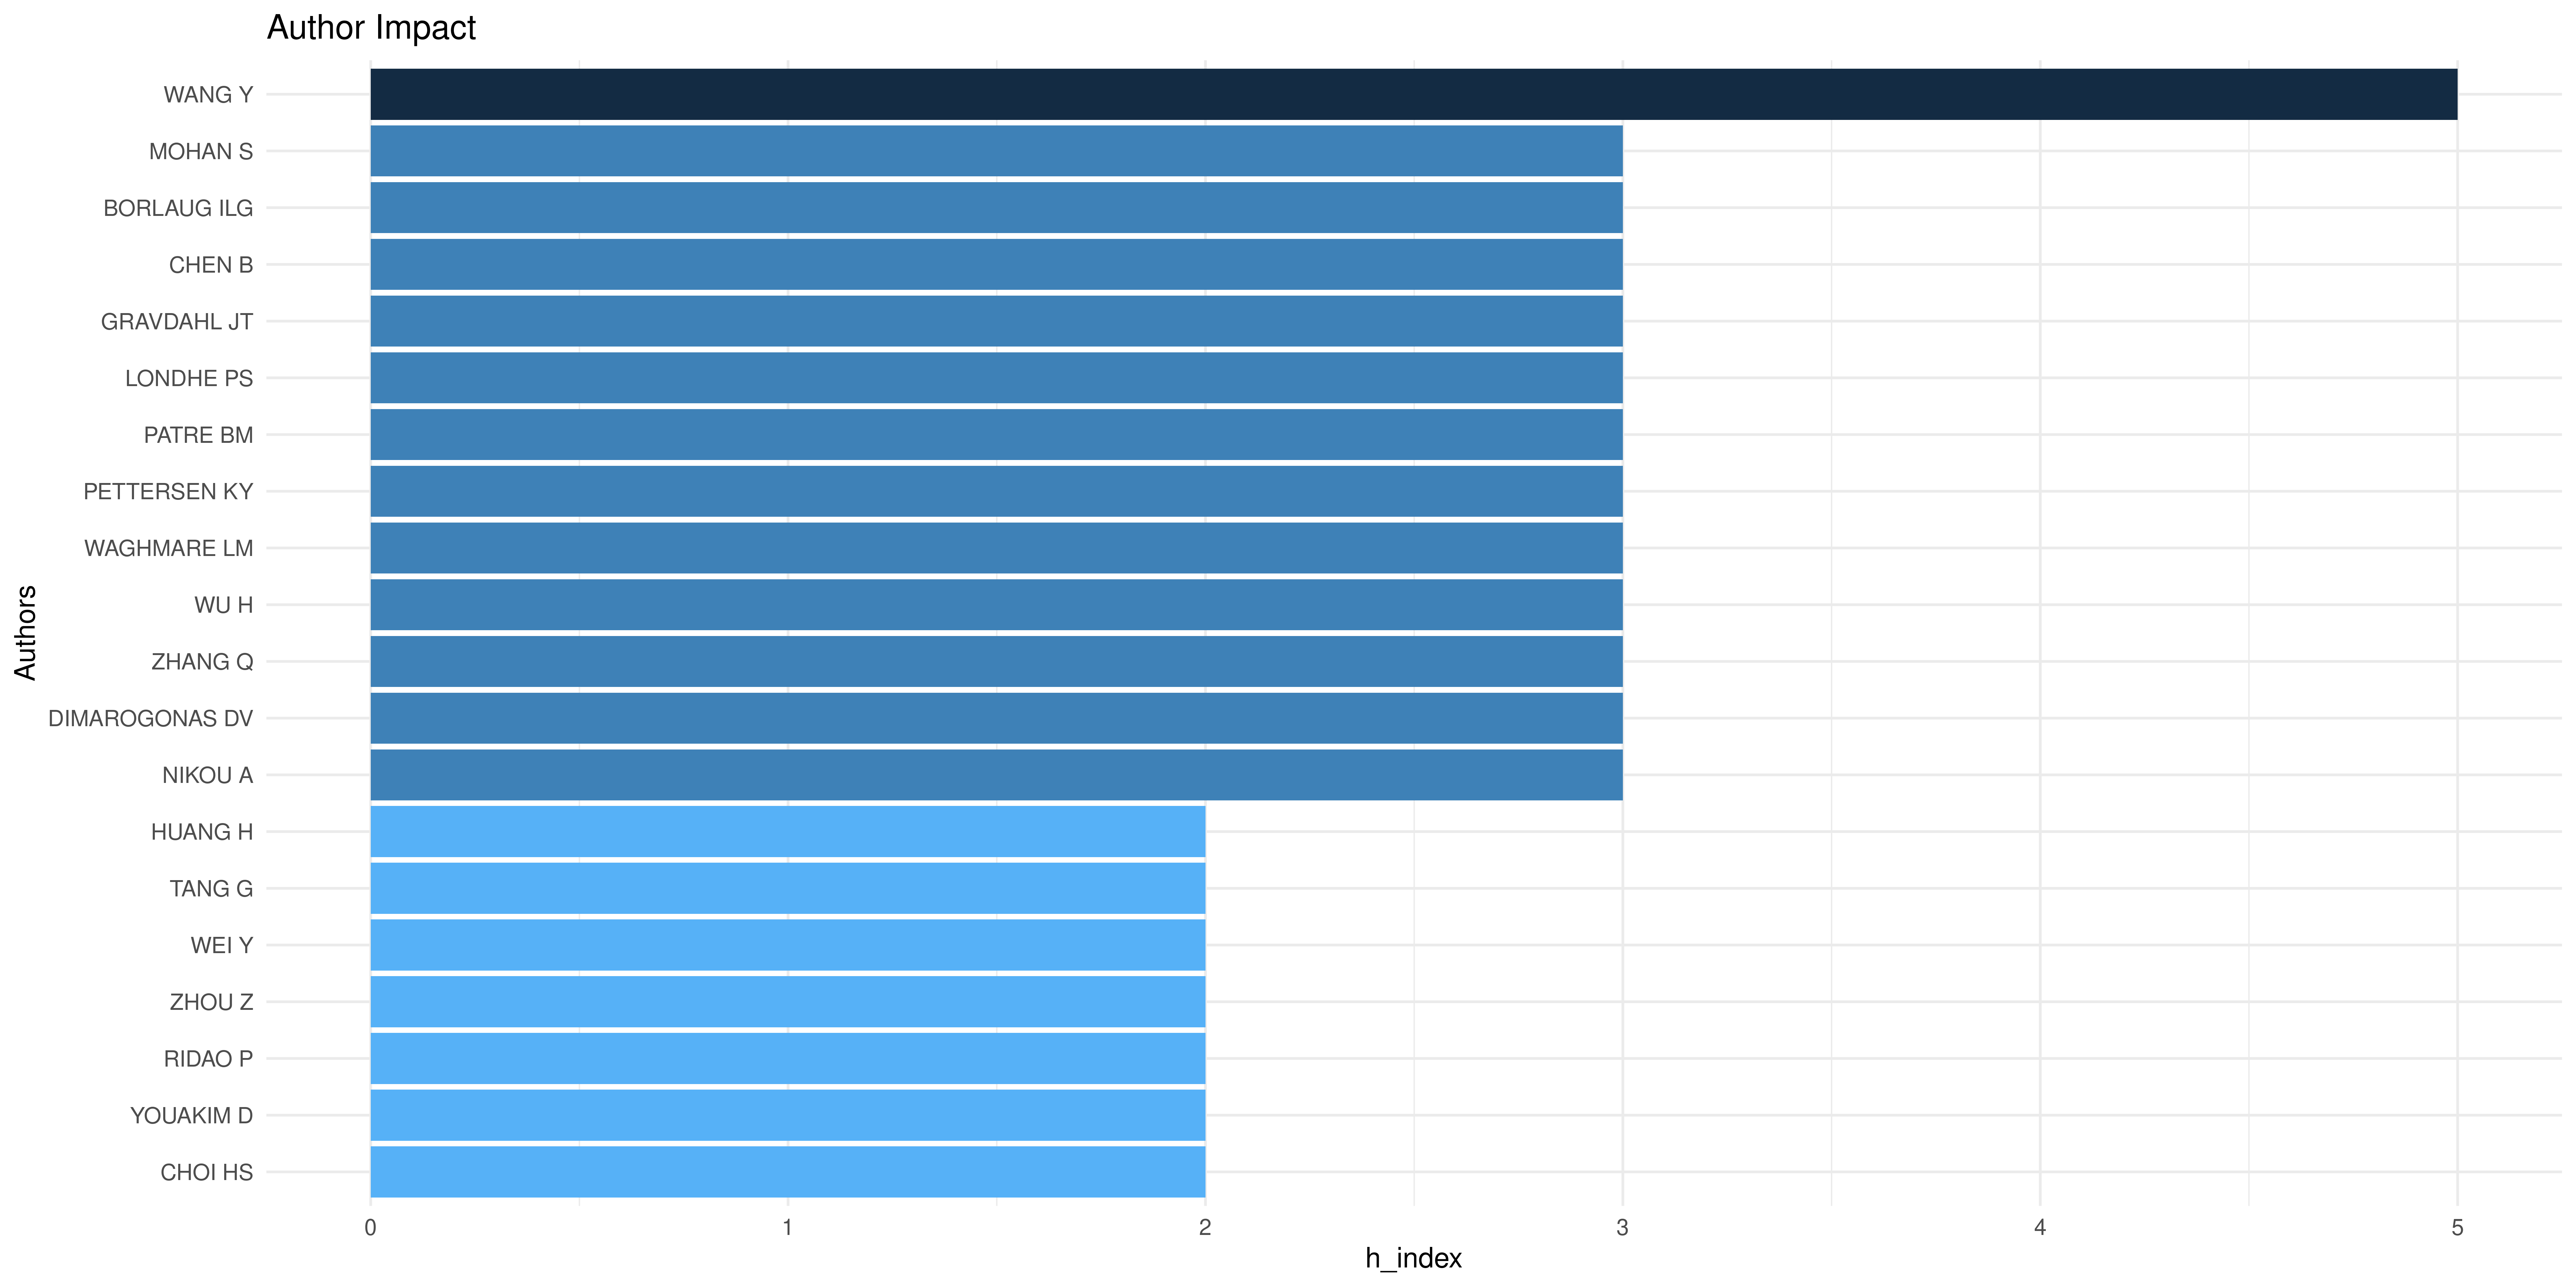
\includegraphics[trim = 0 0 0 0, clip, width=1\textwidth]{AuthorImpact-2021-04-28.png}}

%*----------- notes
    \note[item]{Notes can help you to remember important information. Turn on the notes option.}
\end{frame}
%-
%*----------- SLIDE -------------------------------------------------------------
\begin{frame}[c]{Ciclo Impacto}

    \centering
    \centerline{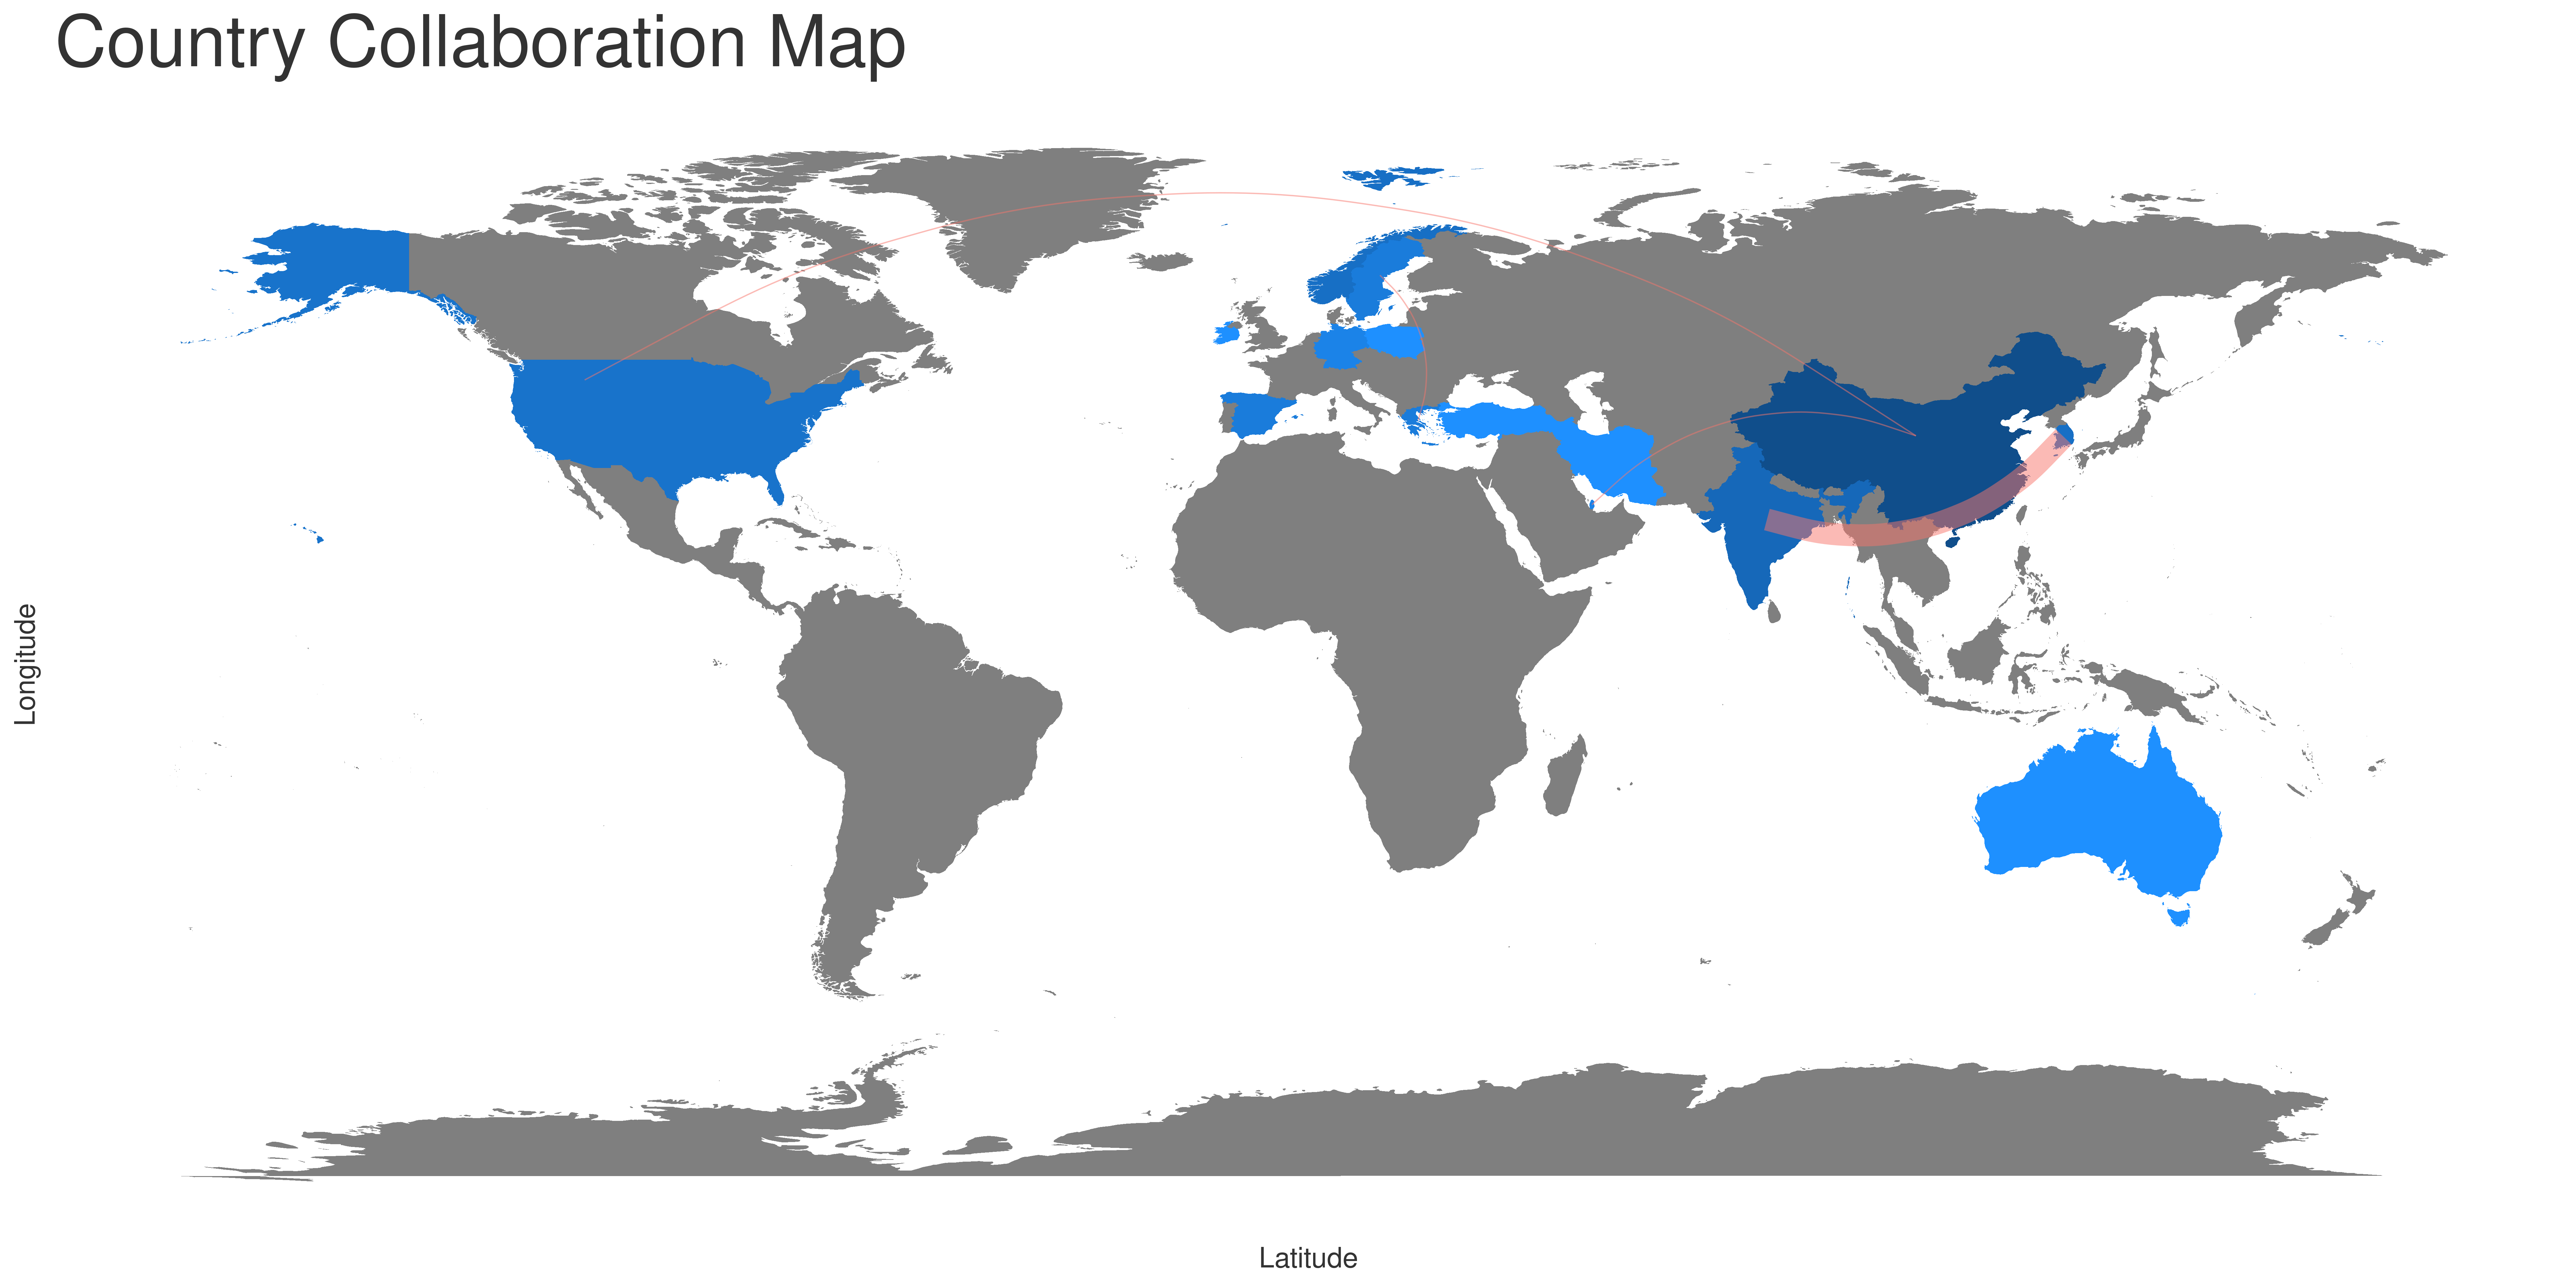
\includegraphics[trim = 0 0 0 40, clip, width=1\textwidth]{CountryCollaborationMap-2021-04-28.png}}

%*----------- notes
    \note[item]{Notes can help you to remember important information. Turn on the notes option.}
\end{frame}
%-
%*----------- SLIDE -------------------------------------------------------------
\begin{frame}[c]{Ciclo Produção}
    \begin{columns}
        \column{.01\textwidth}
        \column{.5\textwidth}
            \centering
            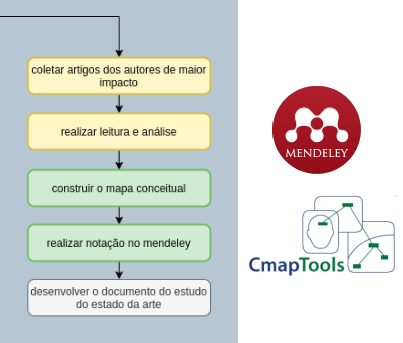
\includegraphics[width=.95\textwidth, trim= 0 0 0 0, clip]{ciclo4.png}
        \column{.5\textwidth}
            Gerar documentos de análise.

            \centering
            \begin{figure}
                     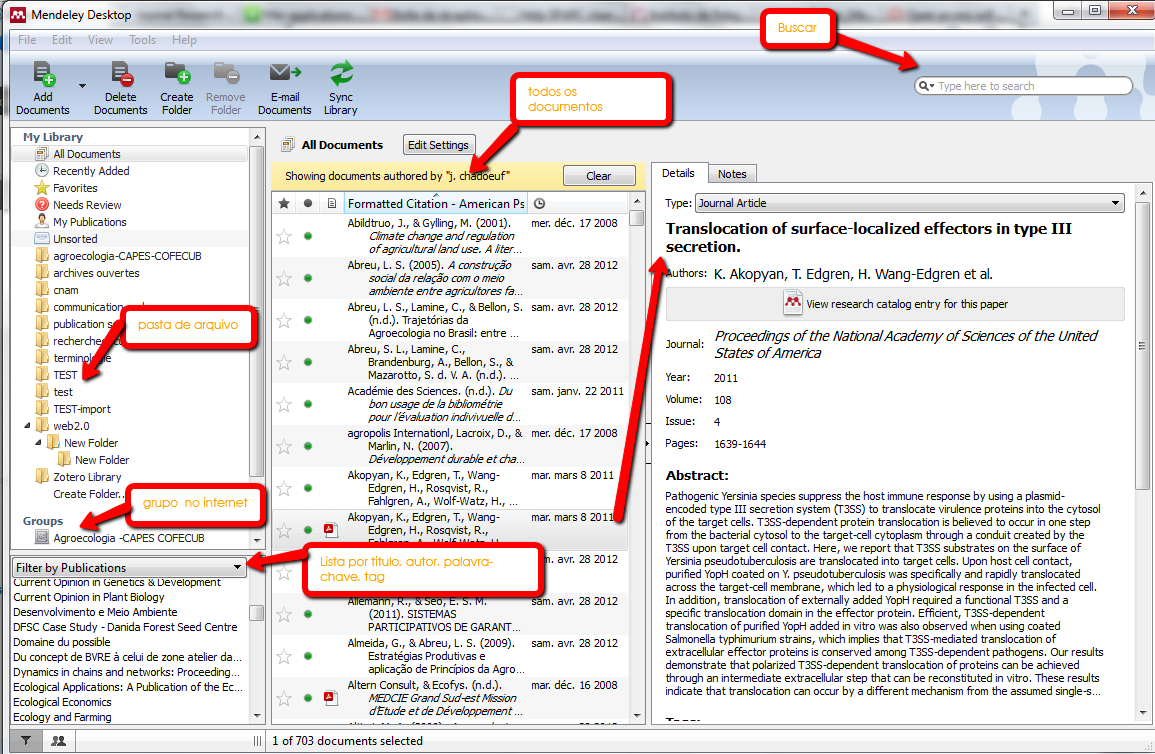
\includegraphics[width=0.7\textwidth]{mendeley.png}
                     \hfill
                     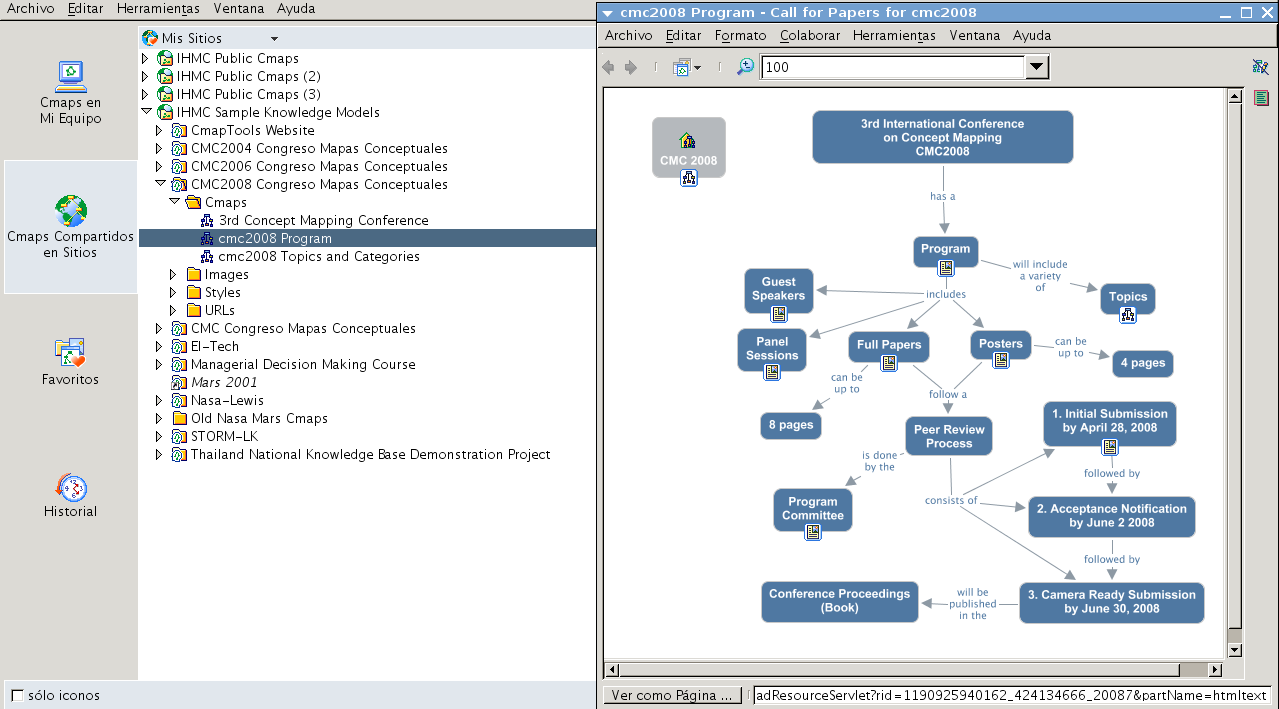
\includegraphics[width=0.7\textwidth]{cmaptools.png}
            \end{figure}
        
    \end{columns}

%*----------- notes
    \note[item]{Notes can help you to remember important information. Turn on the notes option.}
\end{frame}
%-
%*----------- SLIDE -------------------------------------------------------------
\begin{frame}[c]{Ciclo Produção}
    \centering
    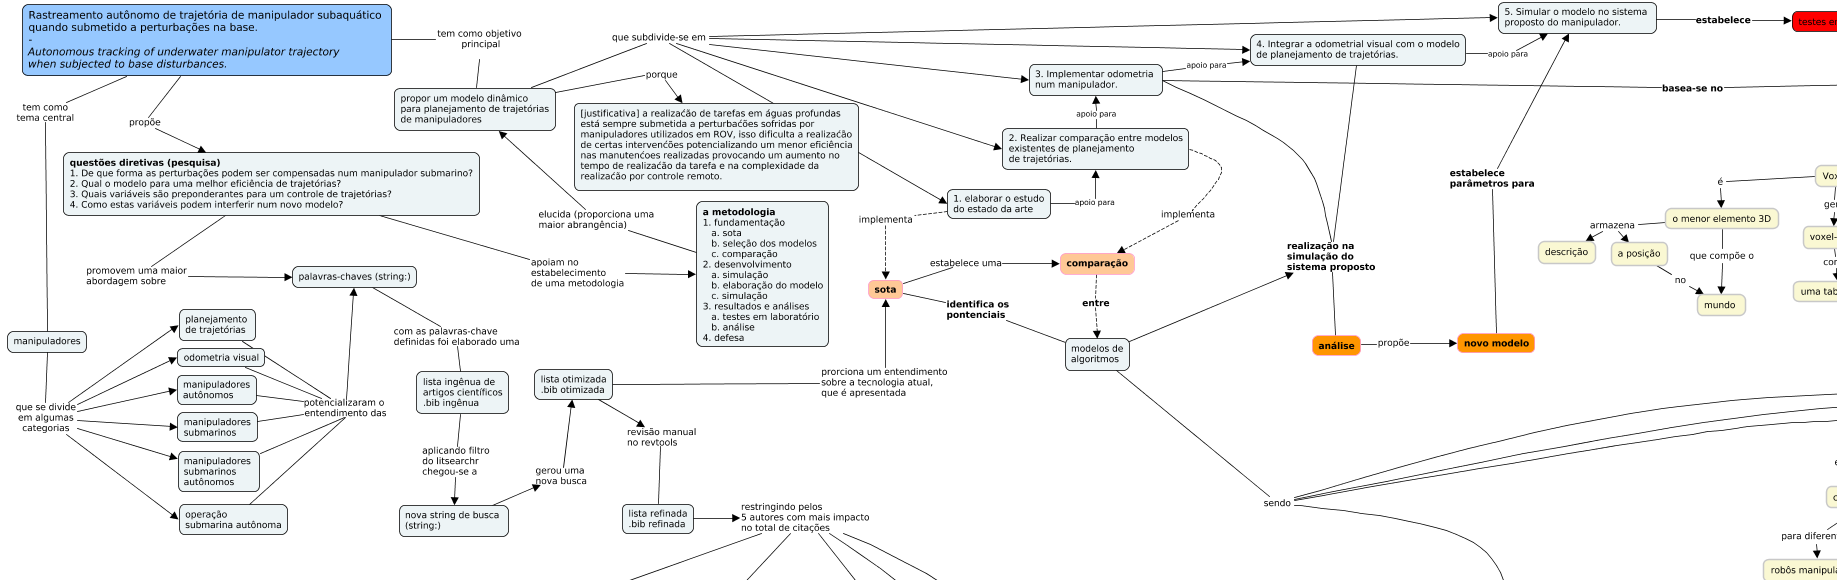
\includegraphics[width=1.5\textwidth, trim = 0 0 300 0, clip]{mapa-conceitual-recorte.png}

%*----------- notes
    \note[item]{Notes can help you to remember important information. Turn on the notes option.}
\end{frame}
%-
%*----------- SLIDE -------------------------------------------------------------
{
\setbeamertemplate{background}
{
\includegraphics[width =\the\paperwidth, clip, trim = 0 0 0 100]{nick-morrison-FHnnjk1Yj7Y-unsplash.jpg}}
%*----------- SLIDE -------------------------------------------------------------
\begin{frame}[t]{} 
\end{frame}
}
%-
%*----------- SLIDE -------------------------------------------------------------
\begin{frame}[c]{}
    \centering
    
\includegraphics[width=.65\textwidth, trim= 0 0 0 0, clip]{github.png}
    
    \vspace*{0.3cm}
    \href{https://github.com/Brazilian-Institute-of-Robotics/bir-mini-method-bili}{link-do-repositório}
%*----------- notes
    \note[item]{Notes can help you to remember important information. Turn on the notes option.}
\end{frame}
%-
%----------------------------------------------------SLIDE------------------
 \begin{frame}[t, allowframebreaks]{References}
 %\frametitle{References}
%\begin{frame}{Reference}
    %\transboxin[duration=1,direction=30]

    % \begin{bibunit}[plain]
    % \cite{guangyi2018research}.
    % %\cite{kanakia2012}
    % %\cite{agostini2007}
    % %\cite{azuma1997survey}
    % \cite{Buss2005}
  
    % \putbib
    % \end{bibunit}
  
    %\bibliographystyle{IEEEtran}
    %\bibliographystyle{IEEEtranS}
    %\bibliographystyle{IEEEbib}
    \bibliographystyle{abntex2-alf}
    %\bibliographystyle{abntex2-num}
    %\bibliographystyle{abnt-alf}
    \bibliography{bibliography} 
    %\putbib

%*----------- notes
    %\note[item]{Notes can help you to remember important information. Turn on the notes option.}
\end{frame}
%
%-
%*----------- SLIDE-BACKUP ------------------------------------------------------
% \backupbegin
% %
% \begin{frame}{Backup}
%     Test
% %*----------- notes-------------------------------
% \note{Notes can help you to remember important information. Turn on the notes option.}
% \end{frame}
% %-
% \backupend
% %-
%*----------- QUESTIONS ---------------------------------------------------------
\begin{frame}[c,plain]
    \lastpage{
        \begin{center}   
            {\usebeamerfont{title} Questions?}\\[3ex] 
            %\hspace{1.5cm} 
            marcoreis@fieb.org.br
        \end{center}
    }
    
%*----------- notes---------------------------------
    \note[item]{Notes can help you to remember important information. Turn on the notes option.}
\end{frame}
%*-------------------------------------------------------------------------------
\end{document}